%\title{beavtex}
\documentclass[double,12pt,1in]{beavtex}
\usepackage{graphicx}
\usepackage{rotating} 
\usepackage{tablefootnote}
\usepackage[separate-uncertainty=true]{siunitx} 
\usepackage{svg}
\usepackage{physics}
\usepackage{amsmath}
\usepackage[autostyle, english = american]{csquotes}
\MakeOuterQuote{"}
\DeclareUnicodeCharacter{2009}{\,} 
\title{Interactions between surface acoustic waves and charge carriers in quantum materials}
\author{Dublin M. Nichols}
\degree{Doctor of Philosophy}
\doctype{Dissertation}
\department{Physics}
\depttype{Department}
\depthead{Head}
\major{Physics}
\advisor{Ethan D. Minot}
\submitdate{Submit Date}
\commencementyear{2024}
\graphicspath{ {Figures/} }



\makeatletter
\g@addto@macro\@floatboxreset\centering
\makeatother


\abstract{Abstract}


\acknowledgements{I would like to acknowledge...}


\begin{document}
\maketitle
\mainmatter

%-------------------------INTRODUCTION-----------------------------

\chapter{Introduction}



\section{Objective}

\section{Background and Motivation}

\subsection{Surface acoustic wave sensors}

\subsection{Quantum pumps}

\subsection{Probing and controlling charge carriers in quantum materials}

Surface acoustic waves enable novel probes into phenomena in quantum systems which can not be measured using conventional transport techniques. For example, SAWs were recently used to prove that current-induced modifications of bubble and stripe phases in 2D electron systems are a local phenomenon \cite{friess_current_2018}. Prior transport-based studies into these phases were inconclusive, as they indirectly probed the phenomenon using the voltage drop on the edges of the 2DEs. The direct measurement of this phenomenon accomplished in Ref. \cite{friess_current_2018} was only possible using a global probe with a fixed length scale, which is precisely what a SAW provides. In another work, new insight into the stripe phase at filling factor 9/2 was gained using a combination of SAWs, microwave excitation, and optical detection \cite{kukushkin_collective_2011}. By employing SAWs with a wavelength of \SI{60}{\nano\meter}, the authors were able to probe commensurability effects between the SAW superlattice and quantum Hall stripes. Earlier SAW-based studies provided new insight into the quantum Hall and fractional quantum Hall effect \cite{wixforth_quantum_1986,esslinger_acoustoelectric_1992,esslinger_ultrasonic_1994,kukushkin_collective_2011,willett_experimental_1993} and Wigner crystallization \cite{paalanen_rf_1992} in 2DEs. These works emphasize the incredible strength of SAWs for probing length-scale dependent phenomena in quantum systems. Building on these successes, researchers have begun to explore the potential of interfacing SAWs in the rapidly evolving field of 2D materials.


In 2018, interest in engineered 2D superlattices exploded with the discovery of unconventional superconductivity in twisted bilayer graphene \cite{cao_unconventional_2018}. The birth of the field of "twistronics" added a new knob to turn in the already massive parameter space available for creating bespoke 2D devices. By tuning the twist angle between two sheets of graphene (and thus the periodicity of the moiré superlattice), bilayer graphene can not only exhibit superconductivity, but also correlation-induced insulating states, magnetism, quantized anomalous Hall states, and many more \cite{andrei_graphene_2020}. In 2D semiconductors, which exhibit exciton dynamics that are of great interest for next-generation electronics, tuning the moiré superlattice provides even more control over the spin and valley degrees of freedom \cite{ciarrocchi_excitonic_2022}. While graphene has a lattice periodicity on the order of \SI{0.15}{\nano\meter}, the moiré superlattices in twisted devices have much longer periods, reaching from tens to even hundreds of nm (on the order of nominal SAW wavelengths). Making quality electrical contacts to 2D semiconductors for transport measurements is notoriously difficult \cite{miao_recent_2022}, and contactless probing using SAWs could circumvent these difficulties. Hence, SAWs are an ideal tool for contactlessly probing and controlling quantum phenomena in 2D materials.

Recent works have combined SAWs and 2D materials to great effect. For instance, one work employed SAWs to transport interlayer excitons over long distances in a 2D semiconductor \cite{peng_long-range_2022}. These excitons, which consist of electrons and holes separated in different 2D layers, are difficult to manipulate because they are charge neutral and exhibit no net force under a uniform electric field. However, the spatially- and temporally-periodic electric field of a SAW transports both electrons and holes in the same direction (*****see sec.*****), enabling long-range transport of these interlayer excitons. In another work, SAWs were used as a contactless probe of measuring wave-vector dependent conductivity in ultraclean graphene, establishing the viability of SAW resonant cavities as a probe for quantum transport in graphene \cite{fang_quantum_2023}. These studies have only scratched the surface of what is possible by interfacing SAWs with 2D materials. Many other SAW-induced phenomena in 2D materials have been predicted, but not achieved experimentally \cite{nie_surface_2023}. Therefore, it is imperative to further develop the methods of interfacing SAWs with 2D materials.




\section{Outline}


\chapter{Theory}

\section{Introduction to graphene}

\section{Surface acoustic waves}

A surface acoustic wave (SAW) is an elastic wave that propagates along the surface of a material, with its energy confined to a depth of around one wavelength below the surface \cite{rayleigh_waves_1885}. When a SAW propagates in a piezoelectric substrate, it mechanically stresses the piezoelectric, generating electric fields. In turn, these electric fields generate strain in the substrate. If we coat this piezoelectric surface with a thin film, the SAW feels and responds to electronic and mechanical properties of the film (in this dissertation the thin film of interest is graphene). This interplay between a SAW and its propagation environment make SAWs interesting for both probing phenomena in quantum materials, such as *insert stuff from intro*, and using quantum materials to probe the environment, such as in gas sensors, humidity sensors.

All of these applications utilize the velocity shift and/or attenuation of the SAW as their sensing tool, which vary depending on mechanical and electronic properties of the thin film coating the piezoelectric surface. Also, in this dissertation, I use SAWs to pump charge through encapsulated graphene. Therefore, I need to develop an understanding of SAW propagation in piezoelectric substrates and the interaction of SAWs with the environment in which they are generated. As we will see, a one-dimensional model of longitudinal SAWs is sufficient to develop this understanding. 

I begin this section with a discussion of elastic waves in bulk non-piezoelectric materials and derive the corresponding wave equation. Then, I discuss waves in bulk piezoelectric materials and explore how the effective stiffness of the piezoelectric substrate varies in cases of very low or very high bulk conductivity. Next, I consider the intermediate conductivity case and derive the bulk conductivity-dependent attenuation and velocity shift equations. Finally, I discuss how the velocity shift and attenuation change when the conductivity is located in a thin film on an insulating piezoelectric surface, and how the attenuation drives a DC acoustoelectric current in the thin film. This sets the stage for the later Sec. \ref{AE paper discussion}, where I modify these equations to consider mixed-carrier transport in graphene. The discussion in this section follows that of Refs. \cite{weinreich_acoustodynamic_1956, hutson_elastic_1962, wixforth_surface_1989}, except where noted by additional references.

\subsection{Elastic waves in non-piezoelectric materials}
To understand the propagation of SAWs in piezoelectric materials, we must first understand the constitutive equation of waves in bulk elastic materials. The constitutive equation relates the displacement of an internal element of this elastic material, known as "strain" (a dimensionless quantity), to the internal forces which caused the strain, known as "stress" (dimensions of force per unit area). The relationship between stress and strain determines how elastic waves propagate. Consider an infinitesimal element $dx$ which is deformed to a length $du + dx$ (Fig. \ref{dfield}). Strain, denoted by $S$, is defined by the local change in displacement $du$ relative to the original length $dx$, 

\begin{equation}
    S = \pdv{u}{x}. \label{strain-displacement equation}
\end{equation}
This is a one-dimensional model, so we do not consider shear strains.
\begin{figure}
    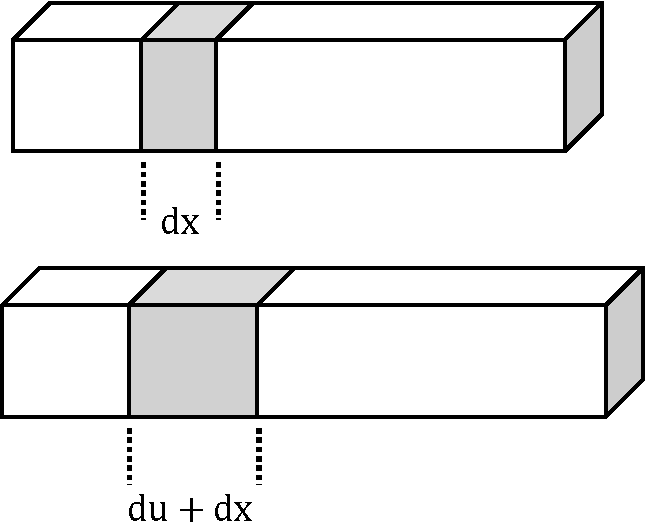
\includegraphics[width = 0.5\textwidth]{displacement field.pdf}
    \caption{A one-dimensional illustration of an element which deforms from length $dx$ to $du + dx$.} \label{dfield}
\end{figure}
Stress, denoted by $T$, is related to strain by the constitutive equation

\begin{equation}
    T = cS, \label{elastic Hooke's}
\end{equation}
where c is the stiffness coefficient, also known as Young's modulus. This is a generalization of Hooke's law, with a linear relationship between strain and stress. Stress $T$ is related to $du$ by 

\begin{equation}
    \pdv{T}{x} = \rho \pdv[2]{u}{t}, \label{stress related to displacement}
\end{equation}
where $\rho$ is the mass density of the material. From these relations, we get an equation for waves in elastic materials

\begin{equation}
    \pdv[2]{u}{t} = \frac{c}{\rho} \pdv[2]{u}{x},
\end{equation}
from which we can readily see that plane waves propagate in this elastic material with a velocity $v_0 = \sqrt{\frac{c}{\rho}}$. This is familiar from travelling acoustic waves in a string: as stiffness increases, waves propagate more quickly, and as mass density increases, waves propagate more slowly. In piezoelectric materials, this intuition holds, with one caveat: the effective stiffness of a piezoelectric material depends on more than just its mechanical properties.

\subsection{Waves in bulk piezoelectric materials}
\begin{figure}
    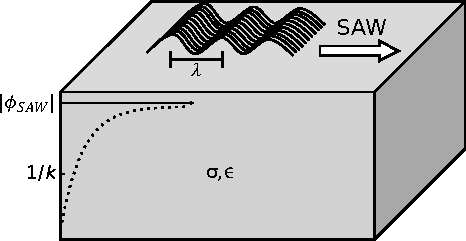
\includegraphics[width=0.5\textwidth]{SAW in bulk semi.pdf}
    \caption{A surface acoustic wave travelling in a bulk piezoelectric material. The SAW amplitude $|\phi_{SAW}|$ is well-known to decay approximately exponentially into the surface, with most of its energy contained within a depth $1/k$ \cite{wixforth_surface_1989}.}
    \label{SAWbulksemi}
\end{figure}

Consider a surface acoustic wave with wave vector $k$ propagating in a bulk piezoelectric material with conductivity $\sigma$ and dielectric permittivity $\epsilon$, shown in Fig. \ref{SAWbulksemi}. In a piezoelectric material, strain creates displacement fields ($D$-fields), and electric fields create stress. This translates to new constitutive equations for waves in piezoelectric materials. For small displacements $u$, these are

\begin{equation} 
    D = eS + \epsilon E \label{Delastic}
\end{equation}
and
\begin{equation} 
    T = cS -eE, \label{Telastic}
\end{equation}
where $e$ is the piezoelectric constant (assumed here to cause electric fields only in the $x$-direction), $c$ is the elastic constant at constant electric field, and $\epsilon$ is the dielectric permittivity at constant strain. Remembering the definition of displacement field $D = \epsilon E + P$, where P is polarization, we can see from Eq. \ref{Delastic} that the strength of polarization in piezoelectric materials scales with the piezoelectric constant $e$, and strain creates a polarization $P = eS$. Equation \ref{Telastic} can be thought of as the same generalized Hooke's law from Eq. \ref{elastic Hooke's}, but with additional stress $-eE$ arising from the piezoelectric effect. 

We are interested in the interaction of SAWs with conducting films, and Eqs. \ref{Delastic} and \ref{Telastic} do not include conductivity (denoted here by $\sigma$). To introduce the effect of conductivity on the constitutive equations, I first consider limiting cases of very high $\sigma$ and very low $\sigma$. In a piezoelectric material with $\sigma = \infty$, $E = 0$ because the material can screen all internal electric fields. The piezoelectric equations of state reduce to 

\begin{equation}
    T = cS
\end{equation}
and
\begin{equation}
    D = eS.
\end{equation}
In this case, our wave velocity is $v_0 = \sqrt{c/\rho}$ (unchanged from before), and the elastic wave propagates in tandem with $D$-fields. This case of a material with very high conductivity is framed by Wixforth et al. as "a material that [to the elastic wave] appears to be non-piezoelectric" \cite{wixforth_surface_1989}.

The next limiting case is that of very low conductivity ($\sigma = 0$). In this perfect piezoelectric insulator, there is no free charge, so Poisson's equation requires that 

\begin{equation}
    \pdv*{D}{x} = 0.
\end{equation}
Rearranging Eqs. \ref{Delastic} and \ref{Telastic}, we find that the wave equation for our piezoelectric insulator is

\begin{equation}
    \pdv[2]{u}{t} = \frac{c}{\rho} (1 + \frac{e^2}{2c\epsilon}) \pdv[2]{u}{x}. \label{wave eqn for insulator}
\end{equation}
Defining $c^* = c(1 + e^2/c\epsilon)$, this describes a wave travelling at a velocity $v^* =\sqrt{c^*/\rho}$. The piezoelectric interaction has caused our effective elastic constant to increase by a factor $e^2/2c\epsilon$! This quantity is known as the "piezoelectric coupling constant", denoted $K^2 = e^2/c\epsilon$, which represents the ratio of coupled piezoelectric energy to total stored energy. "Total stored energy" includes energy stored both in the D-fields (scaling with $\epsilon$) and in mechanical deformation (scaling with $c$). 

$K^2$ varies widely between materials, ranging from $6.4 \times 10^{-4}$ in GaAs \cite{wixforth_surface_1989} to 0.05 in LiNbO\textsubscript{3} \cite{warner_determination_1967}. Stronger piezoelectric interactions (increasing $e$) stiffen the material; conversely, a stronger dielectric (increasing $\epsilon$) softens the material. This effective increase in elastic constant from piezoelectric interactions is known as "piezoelectric stiffening" and has important consequences for interactions between SAWs and charge carriers in thin films, as will be seen shortly. 

Next, we tackle the case of intermediate $\sigma$ — acoustic waves in a piezoelectric semiconductor. In this dissertation, acoustic waves in a piezoelectric semiconductor are particularly interesting because the physics is similar whether $\sigma$ is contained in the bulk piezoelectric or a thin film (like graphene) on an insulating piezoelectric. The current density $J$ in a semiconductor is the sum of the drift and diffusion currents

\begin{equation}
    J = q n \mu E + \frac{\mu}{\beta} \pdv{n}{x}, \label{jdiff}
\end{equation}
where q is the electron charge, $\beta$ is the inverse of Boltzmann's constant times temperature, and $n$ is the carrier density (assumed here to be populated only by electrons). Here, I assume the limiting case where drift current is much larger than diffusion current, so diffusion can be neglected. Differentiating Eq. \ref{jdiff} (neglecting diffusion), we have

\begin{equation}
    \pdv{J}{x} = \mu q \pdv{E}{x}. \label{djdx}
\end{equation}
Using Poisson's equation $\pdv*{D}{x} = -qn$ and the continuity equation $\pdv*{J}{x} = q \pdv*{n}{t}$, Eq. \ref{djdx} becomes

\begin{equation}
    \pdv{D}{x}{t} = -\mu q n \pdv{E}{x}. \label{Ddxt}
\end{equation}
Assuming the $E$ and $D$ fields generated by our SAW take the form of plane waves $E = E_0 \mathrm{exp}(i(kx - \omega t))$ and $D = D_0 \mathrm{exp}(i(kx - \omega t))$, Eq. \ref{Ddxt} becomes

\begin{equation}
    D = -i\frac{\sigma}{\omega} E, \label{DinE}
\end{equation}
where $\sigma = \mu n q$ is the conductivity of the piezoelectric semiconductor. Now we can plug Eq. \ref{DinE} into Eq. \ref{Delastic} to relate $E$ to strain $S$, giving

\begin{equation}
    E = -\frac{e}{\epsilon}\frac{(1-i(\sigma/\epsilon\omega))}{1+(\sigma/\epsilon\omega)^2}S. \label{EinS}
\end{equation}
Finally, the wave equation for a piezoelectric semiconductor can be found by substituting \ref{EinS} into Eq. \ref{Telastic}, giving

\begin{equation}
    T = c(1 + \frac{e^2}{c\epsilon}\frac{(1-i(\sigma/\epsilon\omega))}{1+(\sigma/\epsilon\omega)^2})S. \label{TSsigma}
\end{equation}
Clearly we have a similar equation to Eq. \ref{wave eqn for insulator}, in which our elastic constant is modified by piezoelectric interactions. Here, the value of our elastic constant varies with the ratio $\sigma/\epsilon\omega$. What is this ratio?

One might recognize $\sigma/\epsilon$ as the dielectric relaxation time. If this is not familiar, the derivation is as follows: Assume a free charge distribution $qn$ in our semiconductor. Then, remember that from Poisson's equation and Eq. \ref{djdx} we have

\begin{equation}
    q\pdv{n}{t} = \sigma\pdv{E}{x} = \frac{\sigma q}{\epsilon}n, 
\end{equation}
where $\epsilon$ is the dielectric permittivity of our piezoelectric semiconductor. This differential equation describes an exponential relaxation of carrier density $n \propto \exp{-t/\tau_c}$ with characteristic time $\tau_c = \epsilon/\sigma$. $\tau_c$ is known as the "dielectric relaxation time". For us, it's helpful to think of the dielectric relaxation frequency $\omega_c = \tau_c^{-1} = \sigma/\epsilon$ (sometimes called the "characteristic frequency"), as it appears in \ref{TSsigma}. 

Substituting $\omega_c = \sigma/\epsilon$, \ref{TSsigma} becomes

\begin{equation}
    T = c(1 + K^2\frac{(1-i(\omega_c/\omega))}{1+(\omega_c/\omega)^2})S \label{waveeqn}
\end{equation}
(recalling that $K^2 = e^2/c\epsilon$). Therefore, Eq. \ref{waveeqn} describes a piezoelectric wave travelling at velocity $v = \sqrt{c'/\rho}$, where the modified elastic constant is $c' = c(1 + K^2(1-i(\omega_c/\omega))/(1+(\omega_c/\omega)^2))$.

Most notable in Eq. \ref{waveeqn} is that the effective elastic constant $c'$ depends on the ratio $\omega_c/\omega$. Modulating the ratio between the SAW frequency and the conductivity controls the piezoelectric stiffening. However, $c'$ is complex. What does that mean? To understand the complex elastic constant in Eq. \ref{waveeqn}, consider its differential form,

\begin{equation}
    \pdv[2]{u}{t} = \frac{c'}{\rho} \pdv[2]{u}{x}.
\end{equation}
We can break $c'$ into its real and complex parts. Assume $\sqrt{c'} = \beta + i\gamma$. Then, our plane wave solution becomes

\begin{equation}
    u = u_0 \; e^{(i(kx-k\sqrt{c'/\rho}t))}
    = u_0 \; e^{\gamma kt/\sqrt{\rho}}e^{i(kx - \beta kt/\sqrt{\rho})}. \label{plane wave with loss}
\end{equation}
Examining Eq. \ref{plane wave with loss}, we can readily see that it describes a plane wave with phase velocity 

\begin{equation}
    v = \beta/\sqrt{\rho} = Re{\sqrt{c'}}/\sqrt{\rho} \label{velocity from plane wave}
\end{equation} 
and exponential loss (also known as attenuation) per unit length of 

\begin{equation}
    \Gamma = k \; \mathrm{Im}(\sqrt{c'})/\sqrt{\rho}. \label{attenuation from plane wave}
\end{equation} 
This use of a complex wave propagation constant, where the real and complex parts describe dispersion and attenuation, has been used to describe lossy wave propagation in mechanical, electromagnetic, and piezoelectric materials \cite{holland_representation_1967} \cite[p. 18]{pozar_microwave_2012} \cite{weinreich_acoustodynamic_1956, gonzalez_revisiting_2016}. 

Using Eqs. \ref{velocity from plane wave} and \ref{attenuation from plane wave}, we find the velocity and attenuation of our SAW in a bulk piezoelectric semiconductor to be

\begin{equation}
    \frac{\Delta v}{v_0} = \frac{K^2}{2}\frac{1}{1+(\omega_c/\omega)^2} \label{v_bulk}
\end{equation}
and
\begin{equation}
    \Gamma = K^2 \frac{\pi}{\lambda}(\frac{(\omega_c/\omega)}{1+(\omega_c/\omega)^2}). \label{gamma_bulk}
\end{equation}
Figure \ref{gamma_and_v} shows Eqs. \ref{v_bulk} and \ref{gamma_bulk} plotted with respect to  $\omega_c/\omega$. From this, we can see that the SAW is maximally attenuated at $\omega = \omega_c$ and maximal velocity shift is achieved at $\omega \gg \omega_c$.

\begin{figure}
    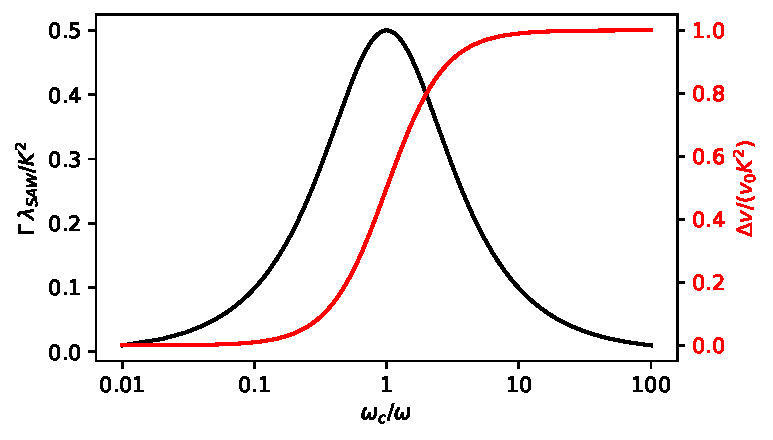
\includegraphics[width=0.8\textwidth]{gamma_and_v.pdf}
    \caption{Eq. \ref{gamma_bulk} (left axis) and Eq. \ref{v_bulk} (right axis) plotted as dimensionless quantities against the ratio $\omega_c/\omega$.}
    \label{gamma_and_v}
\end{figure}
Equations \ref{v_bulk} and \ref{gamma_bulk} are known as the "classical relaxation model" for the acoustoelectric effect. Equation \ref{v_bulk} describes relaxation dispersion, which is common in other acoustic systems \cite{hutson_elastic_1962, rudenko_dispersive_2022} and can be understood as follows: First, the SAW strains the piezoelectric, perturbing the material from its equilibrium state. Then, the piezoelectric relaxes to equilibrium, returning energy to the SAW after a time $1/\omega_c$. However, depending on the time delay between stimulus ($1/\omega$) and response ($1/\omega_c$), this energy returns to the SAW with a phase delay, leading to dispersion and attenuation. In our case, the relaxation time (and thus, $\omega_c$) depends on the conductivity of the piezoelectric semiconductor. 

Equation \ref{ae current density} is fundamental to our investigations into acoustoelectric charge pumping (Sec. \ref{AE charge pumping paper}). However, Eqs. \ref{v_bulk} and \ref{gamma_bulk} describe a bulk material. How do these relations change in the 2D limit? 

\subsection{SAWs propagating in 2D materials}

Equation 2.28 is fundamental to our investigations into acoustoelectric charge pumping
(Ch. 4). However, Eqs. \ref{v_bulk} and \ref{gamma_bulk} describe a bulk piezoelectric material. How do these relations change when the conductivity is located in a thin film on an insulating piezoelectric material? Figure \ref{SAW in thin film} (a) shows the bulk case described by Eqs. \ref{gamma_bulk} and \ref{v_bulk}, in which the SAW's energy and the induced current is contained within a depth $1/k$ of the surface. Therefore, the conductance of the region of the bulk material in which the SAW is propagating is $\sigma' = \sigma/k$. Fig. \ref{SAW in thin film} (b) illustrates a SAW propagating in a material with permittivity $\epsilon$ which is capped by a 2D material of thickness $d$. 

\begin{figure}
    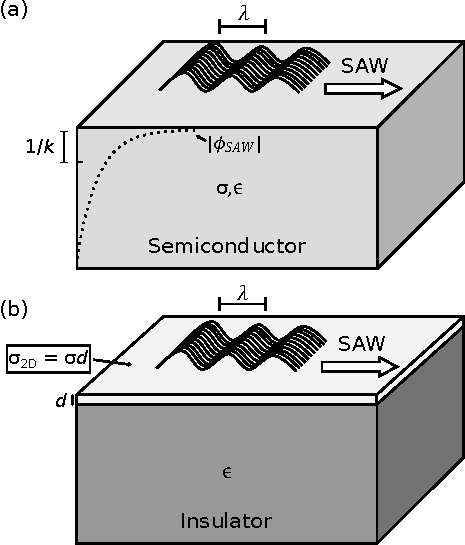
\includegraphics[width = 0.75\textwidth]{SAW in thin film.pdf}
    \caption{(a) A SAW propagating in a bulk material with conductivity $\sigma$ and permittivity $\epsilon$. (b) A SAW propagating in a piezoelectric material with permittivity $\epsilon$ that has been capped by a conductive material of thickness $d$ and sheet conductivity $\sigma_{2D} = \sigma d$.}
    \label{SAW in thin film}
\end{figure}

This can be imagined as compressing the current-carrying region from thickness $1/k$ into a thin layer of thickness $d$ and sheet conductivity $\sigma_{2D} = \sigma d$, where $d \ll 1/k$. Reducing the thickness of the current-carrying region from $1/k$ to $d$ reduces its conductance by a factor of $1/kd$. Therefore, in the 2D case, the dielectric relaxation frequency is also reduced by a factor of $1/kd$, giving $\omega_c = \sigma_{2D}k/\epsilon$. Then, we have
 
\begin{equation}
    \frac{\omega_c}{\omega} = \frac{\sigma_{2D}k}{\epsilon}\frac{1}{\omega} = \sigma_{2D}\frac{k}{\omega \epsilon} = \frac{\sigma_{2D}}{\sigma_M},
\end{equation}
where $\sigma_M = v \epsilon$ is defined as the "characteristic conductivity" of the dielectric environment around the 2D material. Finally, Eqs. \ref{v_bulk} and \ref{gamma_bulk} become

\begin{equation}
    \frac{\Delta v}{v_0} = \frac{K^2}{2}\frac{1}{1+(\sigma_{2D}/\sigma_M)^2} \label{v_2D}
\end{equation}
and
\begin{equation}
    \Gamma = K^2 \frac{\pi}{\lambda}(\frac{(\sigma_{2D}/\sigma_M)}{1+(\sigma_{2D}/\sigma_M)^2}). \label{gamma_2D}
\end{equation}
Similarly to the bulk case (Eqs. \ref{v_bulk} and \ref{gamma_bulk}), the SAW is dispersing and losing energy as it propagates through this conductive 2D material. However, the attenuation and dispersion is frequency-independent, and depends only on the ratio $\sigma_{2D}/\sigma_M$. This leads us an important question: Where does the lost energy of the SAW go? It turns out that this lost energy drives a DC acoustoelectric current that is proportional to Eq. \ref{gamma_2D}.


\subsection{The 2D acoustoelectric effect}

\begin{figure}
    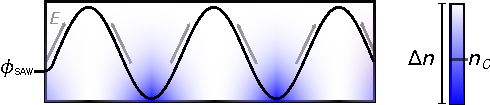
\includegraphics[width = 1\textwidth]{AE current toy model.pdf}
    \caption{A SAW propagating through a thin film with average electron density $n_0$. The co-propagating electric field $E$ (gray arrows) causes a spatially- and temporally-periodic potential (black line), resulting in a spatially- and temporally-periodic perturbation in electron density (blue gradient). The direction of $E$ is a coarse approximation. For a rigorous simulation of the electric field caused by a SAW, see Fig. 1 (c) of Ref. \cite{fang_quantum_2023}.}
    \label{AE current toy model}
\end{figure}

Fal'ko and Iordanskii found that the oscillating electric field that co-propagates with the SAW imparts an effective force on charge carriers, driving a DC current that is proportional to the attenuation $\Gamma$ \cite{falko_acoustoelectric_1993}. In this section, I present the sketch of Fal'ko and Iordanskii's model given in Ref. \cite{esslinger_ultrasonic_1994}, as I found their presentation easier to follow. Figure \ref{AE current toy model} shows a simplified illustration of a SAW propagating through a thin film. As previously discussed, a SAW is accompanied by a co-propagating electric field of the form

\begin{equation}
    E(x, t) = E_0 \mathrm{e}^{i(kx - \omega t)}. \label{SAW plane wave}
\end{equation}
From Ohm's law, $E(x,t)$ creates a local oscillating current density

\begin{equation}
    j(x,t) = \sigma E(x,t), \label{2D AE ohm's law}
\end{equation}
where $\sigma$ is the conductivity of the thin film. This local current density causes  electrons to coalesce in the wells of the SAW potential, as shown in Fig. \ref{AE current toy model}. Assuming that the amplitude of the perturbation in carrier density caused by the SAW (denoted by $\Delta n$) is much smaller than the average carrier density in the thin film (denoted by $n_0$), the periodic carrier density in the SAW takes the form \footnote{If $\Delta n \geq n_0$, the perturbation in $n$ can not be approximated as local, leading to the nonlinear acoustoelectric effect, discussed further in Sec. \ref{nonlinear acoustoelectric effect}.}

\begin{equation}
    n(x,t) = n_0 + \Delta n \mathrm{e}^{i(kx - \omega t)}. 
\end{equation}
Using the continuity equation $\pdv*{J}{x} = q \pdv*{n}{t}$, $\Delta n$ can be written in terms of $E(x,t)$, giving

\begin{equation}
    \Delta n(x,t) = -\frac{\sigma}{q} \frac{k}{\omega} E(x,t) = -\frac{\sigma}{q} \frac{1}{v}E(x,t) \label{delta n modified}
\end{equation}
Next, with $\Delta n \ll n_0$, and remembering that $\sigma = q n \mu$, $\sigma$ can be expanded in terms of $\Delta_n$, taking the form

\begin{equation}
    \sigma(x,t) = \sigma_0 + \pdv{\sigma}{n} \Delta n \mathrm{e}^{i(kx - \omega t)} . \label{sigma modified}
\end{equation}
Now, we can find the DC acoustoelectric current by plugging Eqs. \ref{sigma modified} and \ref{delta n modified} into \ref{2D AE ohm's law} and taking the time average, giving

\begin{equation}
    \begin{split}
        j(x) = \left\langle j(x,t) \right\rangle = \left\langle \left( \sigma_0 + \pdv{\sigma}{n}\Delta n \mathrm{e}^{i(kx - \omega t)} \right) E(x,t) \right\rangle \\
        = \left\langle \left( \sigma_0 - \pdv{\sigma}{n}\frac{\sigma}{q} \frac{1}{v}E(x,t) \mathrm{e}^{i(kx - \omega t)} \right) E(x,t)  \right\rangle \\
        = \left\langle \sigma_0 E(x,t) - \mu  \frac{\sigma}{v} \mathrm{e}^{i(kx - \omega t)}E(x,t)^2 \right\rangle \\
        = - \frac{\mu}{v}\left\langle\sigma E(x,t)^2\right\rangle. 
    \end{split}
    \label{j time averaged}
\end{equation}
One might initially consider the notion of an oscillating $E$-field creating a DC current to be counter-intuitive. However, we can now see that, though $\left\langle E(x,t) \right\rangle = 0$, a DC current arises from the cross-term $\left\langle \sigma E(x,t)^2 \right\rangle$, which corresponds to the time-averaged Ohmic power dissipated by the charge carriers in the thin film. So far, this model considers a local perturbation in $n$ from the SAW; therefore, this cross-term can be thought of as the local dissipation of SAW power by charge carriers in response to the co-propagating electric field. 

Finally, we need to relate Eq. \ref{j time averaged} to $\Gamma$. Remembering that $\Gamma$ describes the loss in SAW intensity per unit length, the SAW intensity can be written in the form

\begin{equation}
    I(x,t) = I_0 \mathrm{e}^{(-\Gamma x)}\mathrm{e}^{(-i\omega t)}.
\end{equation}
Rearranging and differentiating $I$ with respect to $x$, $\Gamma$ takes the form

\begin{equation}
    \Gamma = \frac{1}{I} \pdv{I}{x} = \frac{1}{I}\left\langle\sigma E(x,t)^2\right\rangle. \label{gamma time averaged}
\end{equation}
Then, combining Eqs. \ref{j time averaged} and \ref{gamma time averaged}, the DC acoustoelectric current density becomes

\begin{equation}
    \begin{split}
        j = - \frac{\mu}{v}\left\langle\sigma E(x,t)^2\right\rangle = - \frac{\mu}{v} I\Gamma = - \frac{\mu I}{v} \frac{K^2}{2\lambda}(\frac{(\sigma_{2D}/\sigma_M)}{1+(\sigma_{2D}/\sigma_M)}). 
    \end{split}
    \label{J_2D}
\end{equation}

Equations \ref{v_2D}, \ref{gamma_2D}, and \ref{J_2D} are central to interactions between SAWs and quantum materials. In Sec. \ref{AE paper discussion}, we modify this classical relaxation model, which assumes charge carriers of a single type (Eq. \ref{jdiff}), to describe mixed-carrier transport in graphene.


\section{Surface acoustic wave generation}







%-------------------------Fabrication Methods-----------------------------

\chapter{Methods for fabricating 2D devices}

In 2010, the 2D materials revolution was launched when Geim and Novoselov won the Nobel Prize for their experiments on exfoliated graphene \cite{novoselov_electric_2004}. From the humble beginnings of the ‘scotch tape technique’, the field of has matured to an immense parameter space of layered materials for us to explore. In this lies the greatest strength of 2D materials — we can combine the strengths of different materials to create designer heterostructures. These stacks of 2D materials are called “van der Waals heterostructures”, from the van der Waals force that holds them together. In this chapter, I describe methods for fabricating 2D devices. I begin by describing the best practices that I have found for exfoliation. Then, I discuss my implementation of the dry transfer method for stacking 2D materials to create designer heterostructures. To make contact to these heterostructures, I show two methods — photolithography and electron-beam lithography (EBL) — and compare the strengths and weaknesses of each.


\section{Exfoliation of 2D crystals}

While some groups are investigating large-area 2D growth for use in the next generation of electronics \cite{quellmalz_large-area_2021}, the best devices with the lowest electrostatic disorder are still made using mechanical exfoliation \cite{xin_giant_2023}. Using sticky tape, layered crystals are cleaved 5-10 times, then transferred onto clean SiO2. Flake thicknesses can be determined using optical contrast and verified using atomic-force microscopy (AFM), as shown in \ref*{fig:graphenelayer}.

\begin{figure}[ht!]
    \centering
    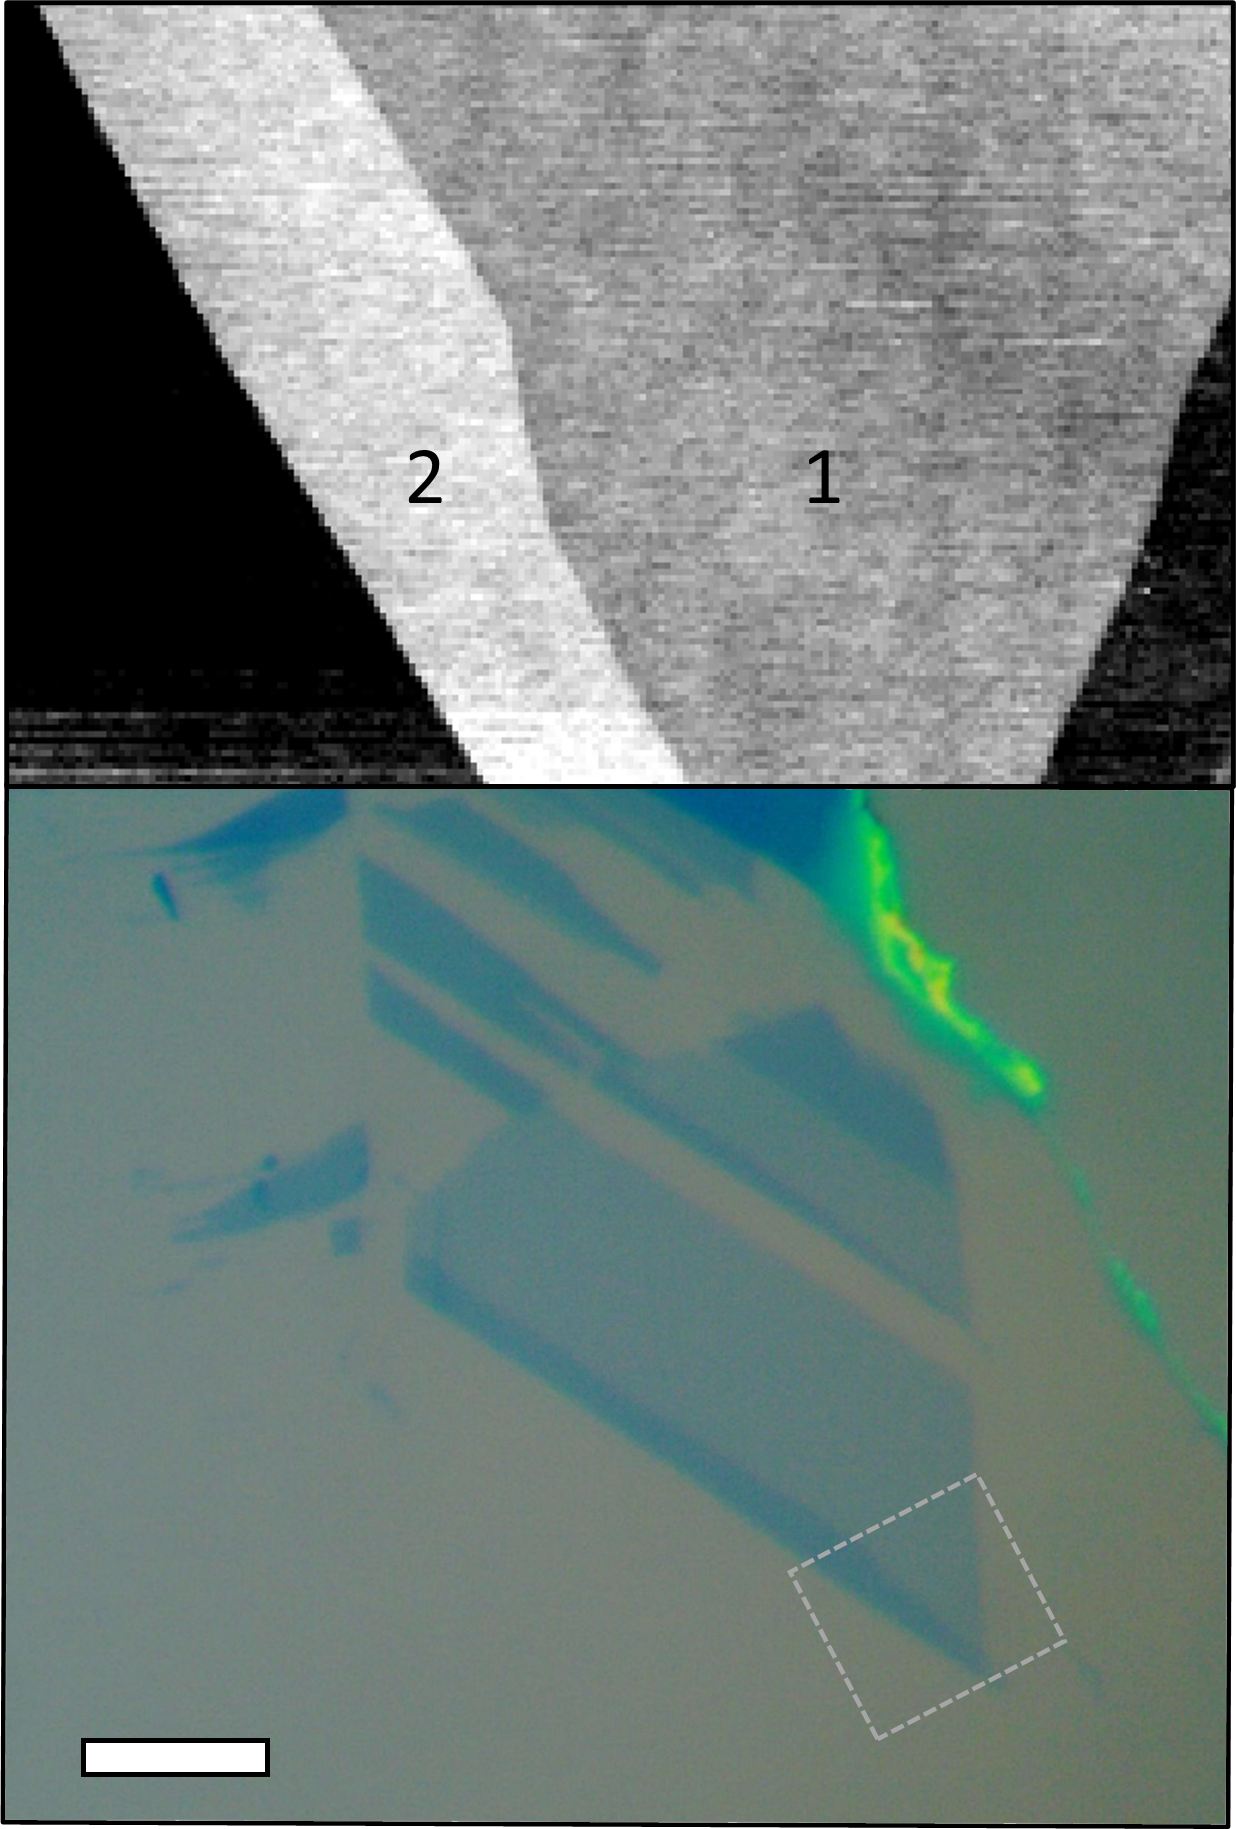
\includegraphics[width = 9cm]{graphene layer comparison.png}
    \caption{Scale bar = 10 $\mathrm{\mu\ m}$}
    \label{fig:graphenelayer}
    
\end{figure}

Exfoliation is a simple process, but getting consistent results can be extremely challenging due to the vast array of variables that affect the process. Different research groups, and even different members in the same group, can have vastly differing opinions on the best methods for exfoliation. These often don’t appear in literature, only being gleaned through personal conversations. Furthermore, every 2D material has different mechanical properties, so the best recipe varies widely between materials. Many of the methods I present in this section were initially learned from the Xu group at University of Washington in 2017, and from the Xu and Yankowitz groups in 2023, then modified from my personal experience. In this section, I give my recommended practices for exfoliating graphene, hBN, and MoS2 onto SiO2. At the end of the section, I summarize this information in Table ***

Exfoliation begins with selecting the tape. The two most widely used tapes are Scotch® Magic™ Tape (“Scotch Tape”) and Nitto Denko SWT20+ wafer tape, (“blue tape”). The main differences between the two are as follows: Scotch tape is stickier and leaves more residue, and blue tape is less sticky and leaves less residue. While blue tape might seem like the obvious choice for the cleanest samples, in a discussion with the Xu group, I learned that they still prefer Scotch tape for graphene, as they feel it gives the largest monolayer flakes. In my experience, I find that Scotch tape does work best for graphene, giving larger-area flakes than blue tape. For hBN, I prefer to use blue tape, as the residue left by scotch tape is similar in color to the hBN flakes, as shown in *this figure*.

\section{Stacking 2D materials: The dry transfer method}


\subsection{PCL cleaning}

\section{Contacts to 2D materials}

\subsection{Photolithography}

In this section, I discuss methods for fabricating 2D devices on piezoelectric substrates using photolithography. One might ask: Why not use electron-beam lithography (EBL)? EBL can achieve higher lithographic resolution than photolithography and allows for bespoke circuit designs to match bespoke 2D heterostructures (see Section ***). For these reasons, EBL is an excellent choice for fabricating 2D devices on SiO2. When performing EBL on a thin (< 0.5\ \SI{3}{\micro\meter}m) layer of insulating SiO2 on conductive Si, the charge buildup from the electron beam can readily dissipate through the thin SiO2. However, piezoelectric substrates like quartz or LiNbO\textsubscript{3} are insulating throughout, leading to charge buildup which deflects the incident electrons and distorts lithographic patterns. To dissipate the charge on insulating substrates, one can either deposit a thin charge dissipation layer on top of the EBL resist with thermal evaporation (often 10-20 nm of Al or Au), which is etched away after exposing the resist, or spin a conductive polymer on the EBL resist which is water-soluble \cite{noauthor_nanolithography_nodate}. These anti-charging layers complicate the fabrication process. Depositing a thin metal charge dissipation layer requires time-consuming thermal evaporation, and removing the metal requires a wet chemical etch. This needs to be repeated for every lithography step. Conductive polymers solve these issues but are prohibitively expensive.\footnote{The most common conductive polymer is ESpacer, which costs \$30,000 per 1 L bottle and expires after 6 months. Recently, an alternative conductive resist has been made available, which is available in smaller quantities \cite{lopez_charge_2019}}  At Oregon State, we can fabricate structures down to \SI{3}{\micro\meter} with photolithography. Unless a device absolutely necessitates smaller feature sizes, it is in our best interest to simplify fabrication and reduce the number of processing steps. However, the motivation for reducing processing steps goes further than just reducing cost and complexity. In my experience, 2D device fabrication is most likely to fail during liftoff. For example, Fig. \ref{fig:hBN lifted} shows a 40 nm flake of hBN transferred onto LiNbO\textsubscript{3} (top panel) which separated from the surface during liftoff (bottom panel), taking 50 nm of metal with it. For these reasons, I chose to use photolithography to fabricate 2D devices on piezoelectric substrates, creating pre-patterned metal contacts on which I transfer the 2DM.
\begin{figure}
    \includegraphics[width = 0.5\textwidth]{hBn lifted off.png}
    \caption{Scale bar = \SI{40}{\micro\meter}}
    \label{fig:hBN lifted}
\end{figure}

When transferring 2DM onto pre-patterned metal contacts, creating a smooth surface is of paramount importance. Therefore, clean liftoff with smooth edges is necessary. For this, I use a bilayer process with a tuned undercut, with S1813 photoresist on top of LOR 3A (“liftoff resist”). The full recipe can be found in *APPENDIX*. Fig. \ref{fig:Liftoff AFM} shows a comparison between single-layer and bilayer liftoff processes in which I attempted to lift off ~25 nm of Cr deposited on SiO2 using electron-beam evaporation. In the single-layer process, metal which coated the resist walls did not lift off with the resist, creating wings that are much larger than the metal thickness. In a bilayer process, the bottom layer of resist develops faster than the top layer, creating an undercut profile that breaks the connection between the metal on the resist walls and the desired pattern. It’s clear that a bilayer process is necessary for prepatterned 2D material contacts. 

\begin{figure}
    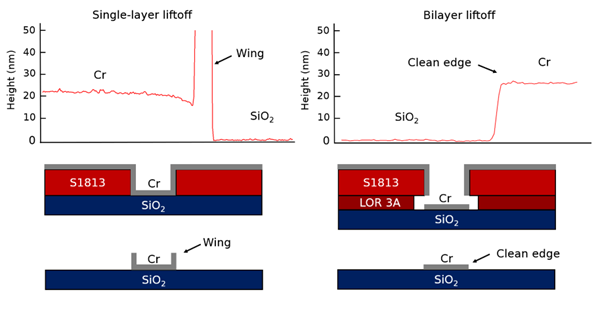
\includegraphics[width = 1\textwidth]{Liftoff AFM.png}
    \caption{AFM trace (top) and schematic (bottom) for single-layer (left) and bilayer (right) liftoff processes of Cr on SiO2/Si.}
    \label{fig:Liftoff AFM}
\end{figure}

The development rate of the LOR can be tuned by varying the bake temperature. A higher temperature bake results in a slower undercut rate, allowing us to optimize the undercut. If the undercut is too large, the top layer of resist will collapse. If the undercut is too small, the metal will not lift off cleanly. I first determined the optimal development time for S1813 as 100 seconds using the interdigitated finger pattern shown in Fig. \ref{fig:hBN lifted} Then, I varied the LOR bake time from 170 C to 190 C and attempted liftoff of 3/20 nm Cr/Au. I found that 180 C was the lowest bake temperature at which liftoff was clean. Figure 2.4 shows a cross-sectional SEM image, in which I confirmed that a 180 C bake and 100 s development creates a ~0.4 \SI{3}{\micro\meter} m undercut.


\begin{figure}
    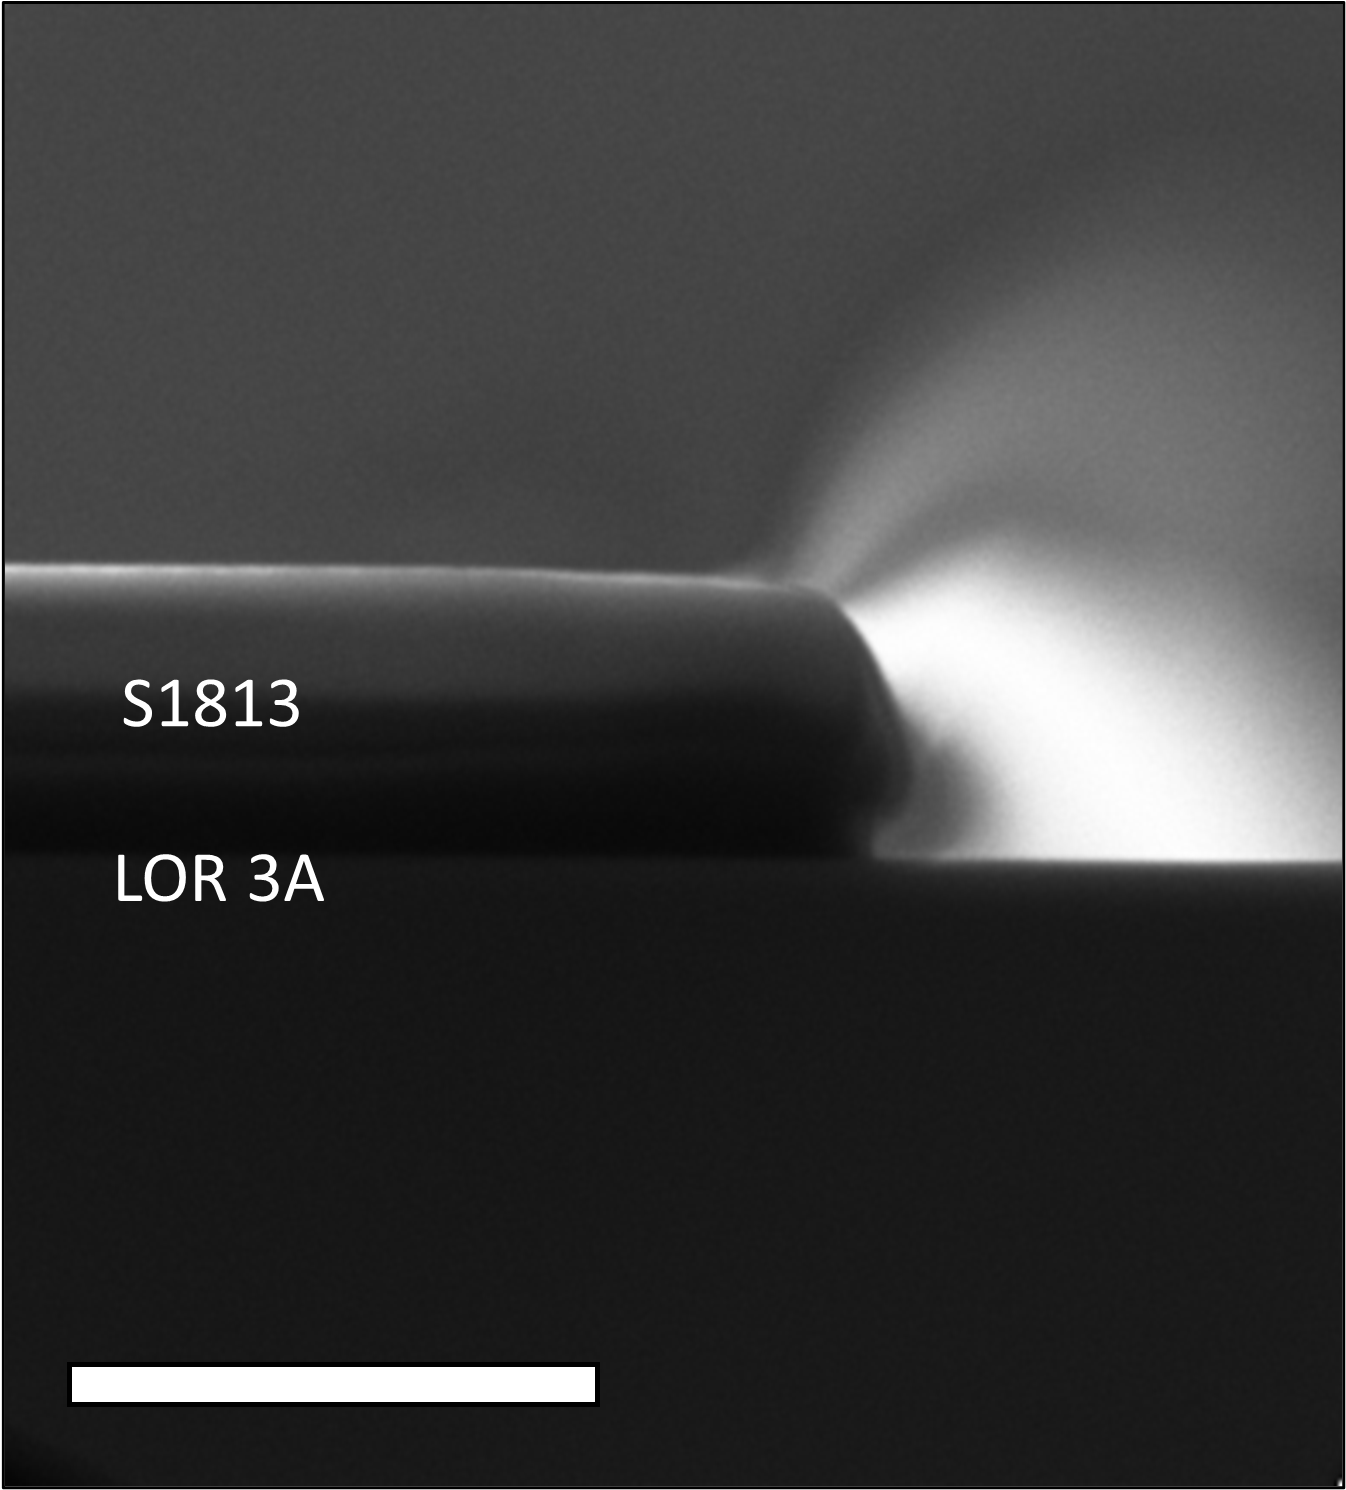
\includegraphics{LOR cross section.png}
    \caption{Cross-sectional SEM image showing bilayer resist process with undercut length $\approx$ \SI{0.4}{\micro\meter}. Scale bar = \SI{3}{\micro\meter}}
    \label{fig:cross-section SEM}
\end{figure}

\section{Electron-beam lithography}

\chapter{Acoustoelectric charge pumping in ultra-clean graphene using surface acoustic waves} \label{AE charge pumping paper}

\section{Abstract}

\section{Introduction} 

\section{Background}

\section{Experiment design}

\section{Results}

\section{Discussion} \label{AE paper discussion}

\section{Conclusion}

\section{Supplementary Material}

\section{Nonlinear acoustoelectric effect in graphene} \label{nonlinear acoustoelectric effect}


Present the paper here (reformat)

% ~~~~~~~~~Flip-chip chapter~~~~~~~~~~

\chapter{Flip-chip design for non-invasive gating of pristine quantum materials}

\section{Introduction}
Lithographic patterning followed by metal deposition is the standard technique to define electrostatic gates; however, the methods of fabricating these devices often involve harsh processing. For example, taking a material to high temperatures — such as during thermal deposition of metals and chemical vapor deposition — can damage sensitive structures by thermal strain (See Appendix on EBL IDT damage from CNT growth processes). Similarly, harsh etching chemicals can introduce impurities and dopants to the surface, affecting electron mobility \cite{beukman_noninvasive_2015}. Electron-beam lithography can also damage pristine surfaces \cite{fink_electron-beam-induced_1990}. To fulfil this need for electrostatically gating a surface while leaving it pristine, the technique of “flip-chip gating” has emerged in recent years \cite{beukman_noninvasive_2015,robertson_non-invasive_2020}. Distinct from the similarly named “flip-chip packaging” technique in semiconductor device processing, flip-chip gating involves flipping the gate chip onto the chip to be gated, allowing a material to be field-effect gated without harsh processing (Fig. 1). This method of flip-chip construction has led to breakthroughs in hybrid quantum systems \cite{chu_creation_2018,satzinger_quantum_2018}.

The air gap between the gate chip and nanomaterial to be gated is of paramount importance for flip-chip devices. As the flip-chip spacing $d$ increases, a capacitive electrostatic gate decreases in strength as $1/d$, and as mentioned in \ref{SAW devices}, most of the energy in a SAW's periodic potential is contained within one SAW wavelength of the surface. As we build higher-frequency SAW devices to interface with nanomaterials, such as for creating quantum pumps that output higher-magnitude quantized current, our flip-chip’s spacing becomes increasingly important. However, most prior works don’t ensure parallel mounting nor directly measure their flip-chip’s spacing \cite{chu_creation_2018,satzinger_quantum_2018,bennaceur_mechanical_2015}, with one work estimating their air gap using capacitance \cite{beukman_noninvasive_2015}, and another roughly estimating their air gap by comparing to similar non-flip-chip devices \cite{bennaceur_mechanical_2015}. In this chapter, I present a flip-chip platform that does not rely on external mounting pressure, and allows for characterization of the flip-chip air gap in multiple areas to determine parallel mounting. Instead of springs or tension arms, my design uses hard-cured varnish and etched Si spacers to hold a precise air gap. I benchmark this platform by building a flip-chip capacitor using photolithography, deep reactive ion etching (RIE), and a homebuilt flip-chip assembly station. I verify the spacing between the two chips with two independent methods — capacitance, and reflectance spectroscopy — and evaluate the feasibility of a flip-chip without external mounting pressure.


\begin{figure}
    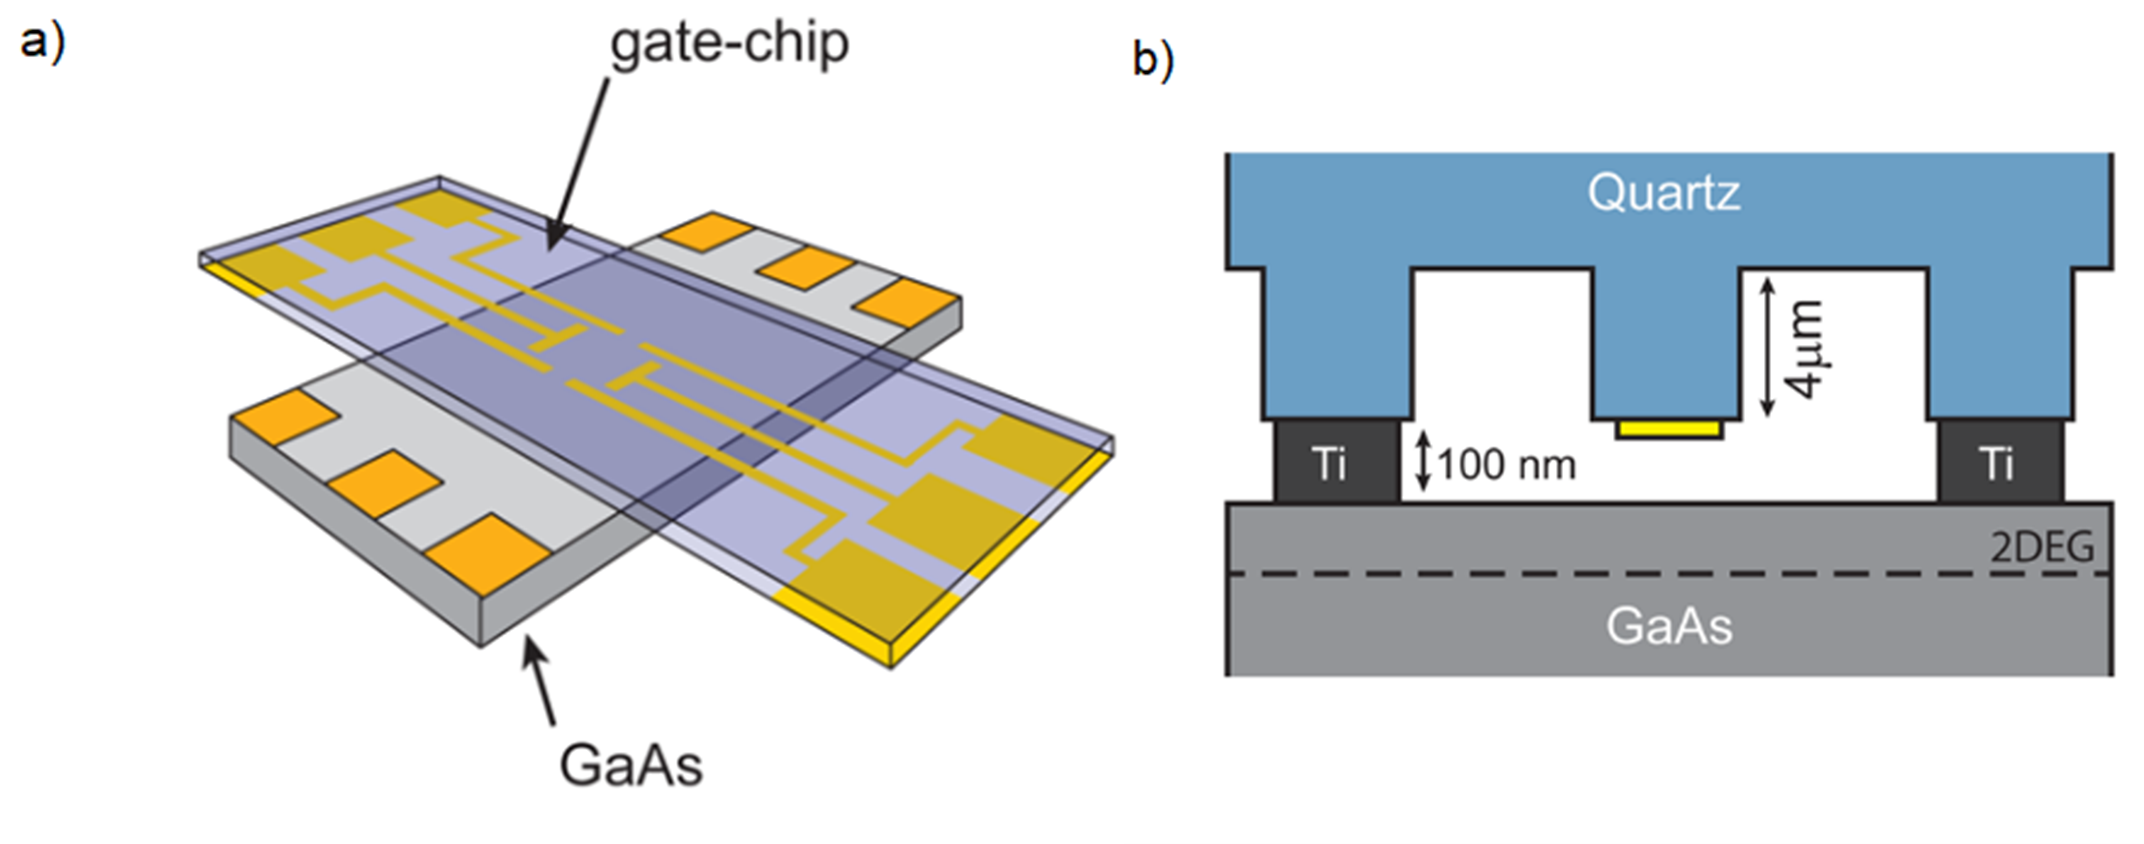
\includegraphics[width=1\textwidth]{Flip-chip design from Ref 1.png}
    \caption{Flip-chip design from \cite{beukman_noninvasive_2015}. (a) The upper gate-chip is printed on quartz to allow alignment with the lower GaAs chip. The lower chip’s gates are attached by micro soldering to preserve the pristine GaAs surface’s ultrahigh electron mobility. (b) Side view of the stacked chips. The gate (yellow) and GaAs are separated by 100 nm using patterned Ti posts.}
    \label{}
\end{figure}

\section{Measuring flip-chip spacing using interference spectroscopy}

The first method I use to measure the air gap between two chips is interference spectroscopy. Using a laser with a spot size $<$ \SI{1}{\milli\meter}, I can not only measure the central air gap, but probe various spots on the flip-chip to determine if the two chips are parallel. Figure \ref{InterfSpec} shows the optical setup used in the interference spectroscopy measurement.


\begin{figure}
    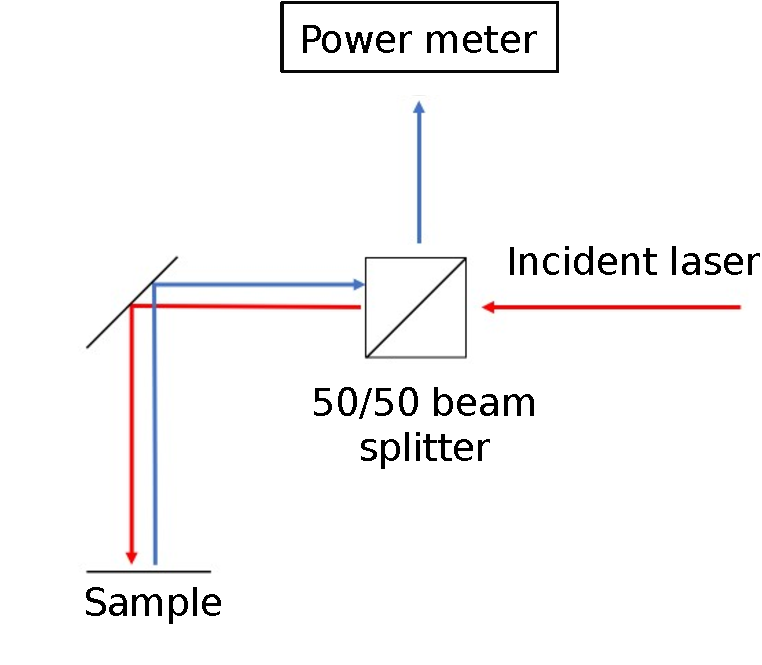
\includegraphics[width = 0.5\textwidth]{Interference spectroscopy.pdf}
    \caption{The interferometer setup used to measure the reflectance of a sample. Incident wavelength is scanned using a Labview-controlled monochromator and plotted against measured reflected power. The colors indicate incident light (red) and reflected light (blue).}
    \label{InterfSpec}
\end{figure}

To correct the reflectance spectrum for wavelength-dependent power fluctuations and substrate effects, I measure a reference spectrum using a bare Si substrate, then subtract this reference spectrum from the measured interference spectrum. Then, I determine the flip-chip air gap by hand-fitting to a model spectrum calculated with Filmetrics’s online thin-film modelling calculator. 

As a first test, I spun a PMMA 495 A11 solution on a Si chip at 2500 RPM for 60 seconds. According to the manufacturer's spin curves, the PMMA layer should be $\approx$ \SI{1000}{\nano\meter} thick. Then, I used the process described in \ref{FCfab} to glue a quartz chip on top to create the Si-PMMA-quartz stack shown in the inset of Fig. \ref{PMMAqzspec}. Figure \ref{PMMAqzspec} shows the corrected reflectance spectrum of this Si-PMMA-quartz stack versus the reflectance calculated with the Filmetrics model.


\begin{figure}
    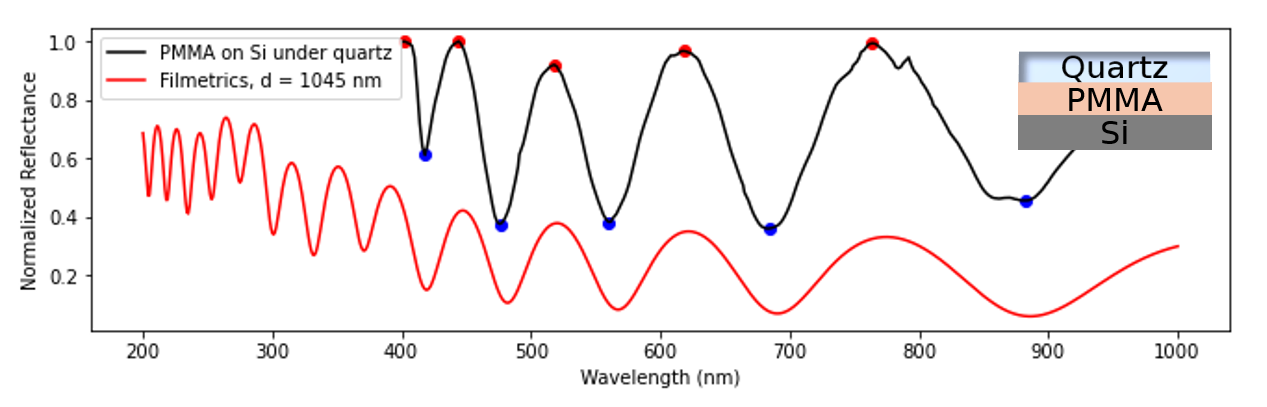
\includegraphics[width=1\textwidth]{qzPMMAsi stack spec.PNG}
    \caption{Corrected measured reflectance of a Si-PMMA-quartz stack compared to the Filmetrics reflectance calculation with \SI{1045}{\nano\meter}-thick PMMA.}
    \label{PMMAqzspec}
\end{figure}

The peaks and troughs of the measured reflectance spectrum are consistent with a PMMA thickness of \SI{1045}{\nano\meter}, close to the predicted spun PMMA thickness, verifying the validity of this method.



\section{Flip-chips with no spacers} \label{FCfab}
Figure *** shows a diagram of my home-built flip-chip assembly station. I designed the holder arm with a "tuning fork" structure (Fig. *** b) which allows me to look through the quartz chip to align structures on the top and bottom chips. For all the flip-chips described in this chapter, I used the following assembly process: To create the top and bottom chips, I coated fused quartz and bare p-doped Si wafers (University Wafer) with S1813 photoresist to protect them during the dicing process, then diced the Si into \SI{7}{\milli\meter} $\times$ \SI{12}{\milli\meter} rectangles and the quartz into \SI{4.5}{\milli\meter} $\times$ \SI{12}{\milli\meter} rectangles using a DISCO DAD 3220 wafer dicing SAW. Immediately prior to gluing the chips together, I removed the photoresist by soaking in a \SI{60}{\celsius} Remover PG bath for 15 minutes, followed by spraying with acetone and isopropyl alcohol and drying with dry N2. Then, I cleaned both chips by submerging them in acetone and rubbing for 20 seconds with a Rubystick T-21 swab to remove any dust \cite{lane_integrating_nodate}. Next, using PDMS strips, (Gel-Pak), I mounted them to the homebuilt flip-chip mounting station as shown in Figure ****. 

Figure \ref{FCnospacerIF} shows an optical image of a flip-chip during alignment. First, I align the edges of the top and bottom chip to ensure they are perpendicular. Then, I slowly lower the z-stage to bring the chips into contact, watching for interference fringes. As the flip-chip spacing becomes smaller, the interference fringes change. Once the top chip contacts the bottom chip, the spacing will not change as I lower the z-stage, so the interference fringes will remain static. This is how I determine that the two chips are in contact. Once the top and bottom chips are in contact, I glue the two chips together by putting two small beads of GE 7031 varnish at the edges. I hard-cure the varnish using a heat gun at 200 C for 5 minutes, holding the heat gun 20 cm from the chip. I also attempted to use photoresist to glue the chips together, as in Ref. \cite{beukman_noninvasive_2015}, but it was difficult to avoid photoresist flowing between the sandwich due to the capillary effect (see Appendix \ref{additional flip-chip tests}).

As a first check, a flip-chip's cleanliness can be assessed by viewing the interference fringes (Newton's rings) visible through its quartz top. Figure \ref{newtonsrings} illustrates the pattern of interference fringes expected from different surface topographies. If the two surfaces are parallel, the rings will be parallel (Fig. \ref{newtonsrings} (A)). Similarly, if a large piece of dust comes between the two surfaces, a point with many small concentric fringes will be visible, curving towards the point which the dust bridges the air gap (Fig. \ref{newtonsrings} (B)). This method was used in \cite{bennaceur_mechanical_2015} to confirm that no large dust particles settled between the two sides of their flip-chip.


\begin{figure}
    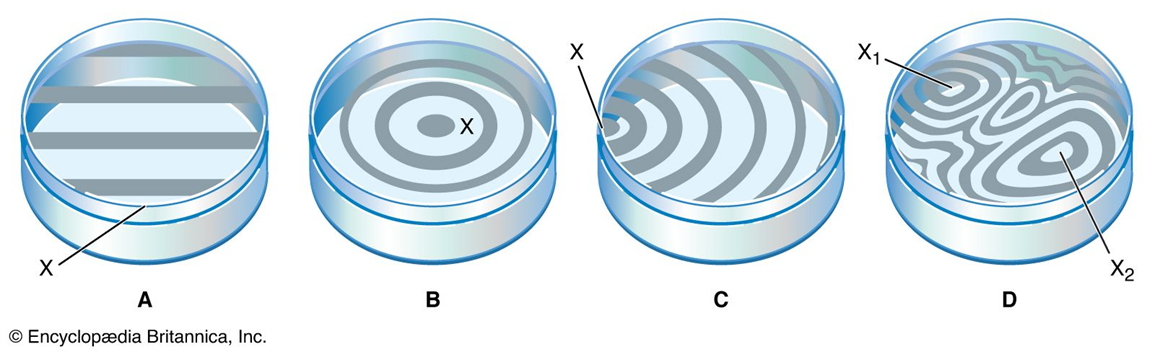
\includegraphics[width=1\textwidth]{newtonsrings.png}
    \caption{From \cite{noauthor_newtons_nodate}}
    \label{newtonsrings}
\end{figure}



\subsection{Smallest achievable air gap} \label{smallest achievable air gap}
Before attempting to control the air gap between two chips, I first need to determine the smallest air gap that I can achieve between two clean chips. Figure \ref{interference sandwich} (a) shows a flip-chip constructed from pristine quartz and Si chips using the method described in Sec. \ref{FCfab}. I performed three interference spectroscopy measurements on this chip — one in the center, and one on each edge — to determine if the chips are mounted parallel to each other.


\begin{figure}
    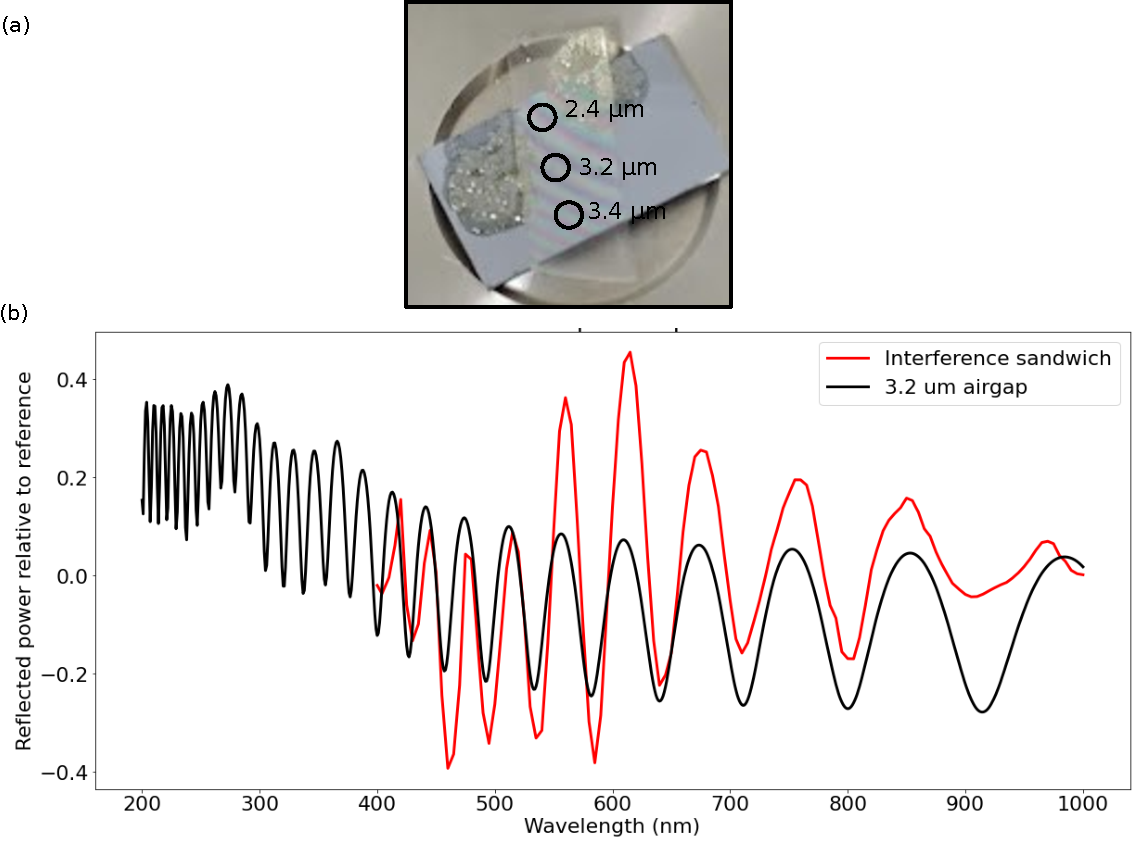
\includegraphics[width=1\textwidth]{interference sandwich image and spectrum.pdf}
    \caption{(a) A flip-chip with no spacers made from quartz and Si. The three circles indicate the spots at which I directed the laser for interference spectroscopy air gap measurement. (b) The reflectance spectrum from the central spot compared to the Filmetrics model with a \SI{3.2}{\micro\meter} air gap.}
    \label{interference sandwich}
\end{figure}

The air gap measurement confirms that one side of the flip-chip is $\approx$ \SI{1}{\micro\meter} closer than the other side. Note that the interference fringes curve towards the side with the smallest spacing, as expected. I constructed two other flip-chips with no spacers, and the smallest spacing I could achieve was the \SI{2.4}{\micro\meter} side of the flip-chip shown in Figure \ref{interference sandwich}. I was not able to determine the exact reason for this limit. When I observed visible dust between the chips, I uncoupled the flip-chip and cleaned the Si and quartz chips. No visible dust is present between the flip-chip shown in Fig. \ref{interference sandwich}. However, unseen dust of size $\approx$ \SI{2.4}{\micro\meter} could be present. The air gap limit could also arise from thickness variation over the surface of the quartz and Si wafers. Ref. \cite{bennaceur_mechanical_2015} attributes their minimum achievable flip-chip spacing (fabricated in a class-100 clean room) of 50 to \SI{200}{\nano\meter} to the top and bottom chips not being perfectly flat across the contact area. We did not buy special $<$ \SI{1}{\micro\meter} total thickness variation Si wafers from University Wafer; furthermore, they do not quote the thickness variation of their fused quartz wafers. From these flip-chips with no spacers, I determine \SI{2.4}{\micro\meter} to be the lower bound for the air gap that I can reasonably achieve with etched Si spacers, and use this to inform my flip-chip design in the next section.


\section{Flip-chip capacitor with deep RIE-etched Si spacers} \label{FC SIspacer}
In the previous section, I determined that the smallest spacing that I can reasonably achieve between two pristine chips is \SI{2.4}{\micro\meter}. However, this does not exclude the possibility of bringing the gate chip closer to our nanomaterial in a small area while leaving most of the flip-chip spaced by $\geq$ \SI{2.4}{\micro\meter}. A two-tier etch has previously been used to achieve a narrow central spacing of $<$ \SI{1}{\micro\meter} while leaving a larger air gap between most of the area of the flip-chip \cite{beukman_noninvasive_2015}. This reduces the likelihood of dust becoming sandwiched in-between the chips and preventing close spacing. 

Figure \ref{twotier} shows the two-tier deep reactive ion etch (RIE) process that I use to create pillars that define the flip-chip spacing. I first print 50 $\times$ \SI{50}{\micro\meter} Cr squares with center spacing \SI{360}{\micro\meter} and thickness \SI{150}{\nano\meter} on a p-doped Si substrate using photolithography (Figure \ref{twotier} (1)). This Cr serves as an etch mask for the deep RIE. Then, I use the SI etch recipe described in \ref{Si RIE recipe} and an Oxford Plasmalab 100 plasma etch system to etch \SI{460}{\nano\meter} into the Si (Figure \ref{twotier} (2)). This first etch defines the center spacing of the flip-chip. Next, I print the capacitor structure using photolithography and metallization of \SI{150}{\nano\meter} Cr, consisting of a 750 $\times$ \SI{750}{\micro\meter} square center pad and \SI{50}{\micro\meter} wires that extend to the edges of the chip (Figure \ref{twotier} (3)). I fabricated this same capacitor structure on both the Si and quartz chips (Figure \ref{twotier}(b)). The long wires allow me to make electrical contact to the central pad of the capacitor when the two chips are sandwiched together Then, I etched the final \SI{5}{\micro\meter} into the Si Figure \ref{twotier} (4). For both Si etches, I determined the exact etch depth using AFM. Figure \ref{FCcap during alignment} shows the flip-chip capacitor during alignment. I assembled the flip-chip capacitor using the process described in Sec. \ref{FCfab}. 
 

\begin{figure}
    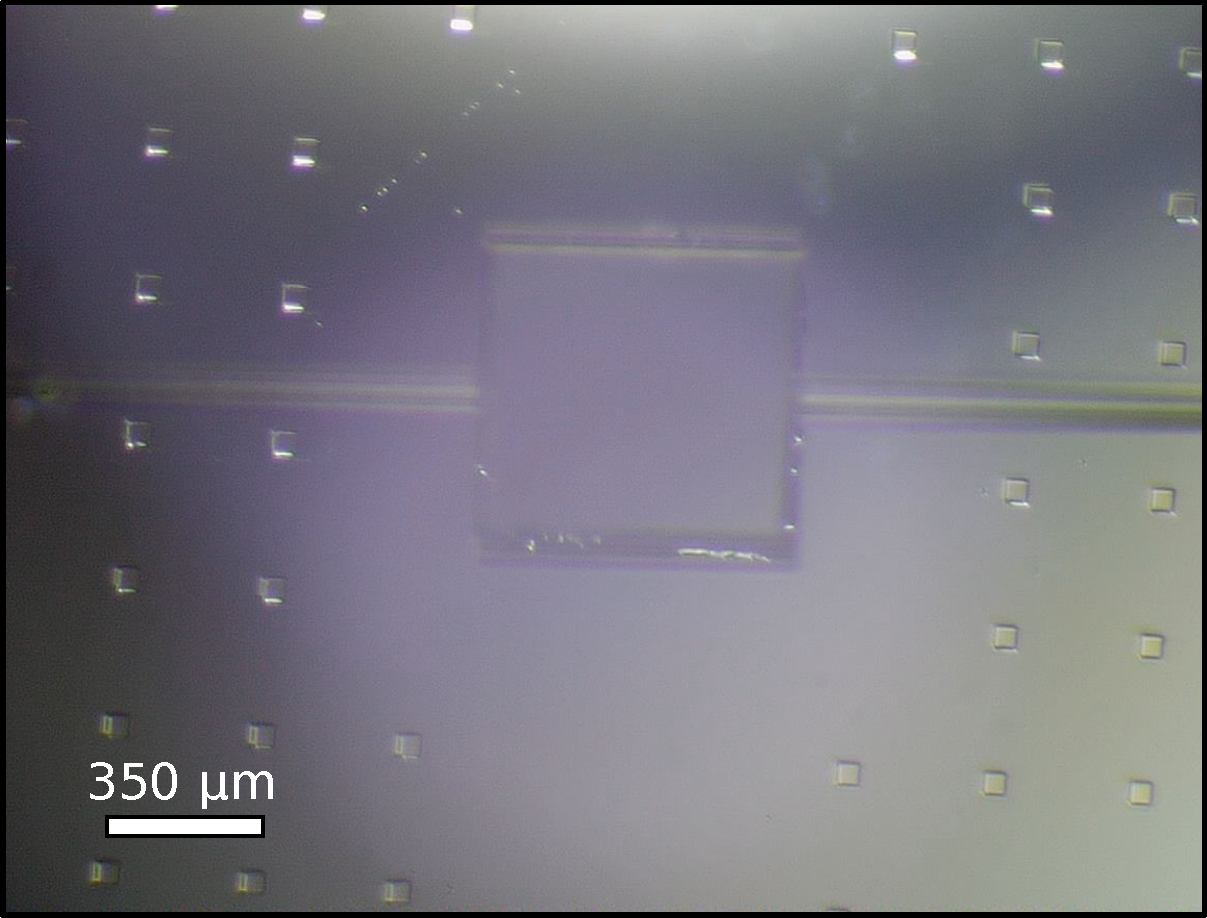
\includegraphics[width = 0.5\textwidth]{FCCap during alignment.pdf}
    \caption{View through the microscope camera during initial alignment of the flip-chip capacitor (the top and bottom chips are still far from each other, so no Newton's rings are visible).}
    \label{FCcap during alignment}
\end{figure}

\begin{figure}
    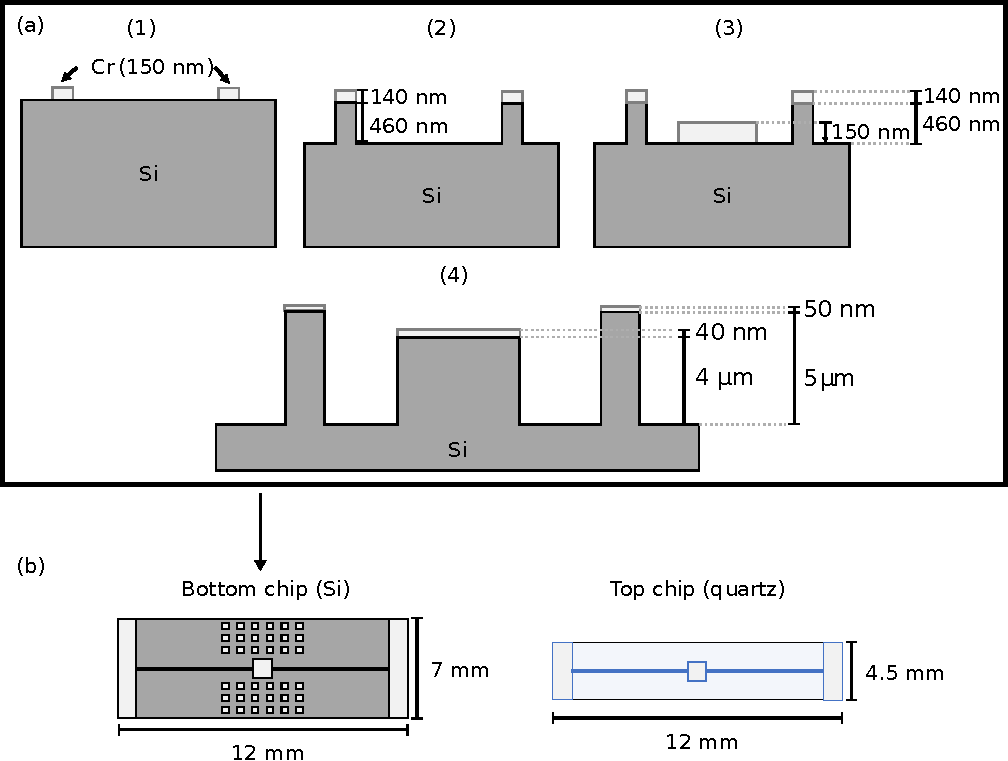
\includegraphics[width=1\textwidth]{Two-tier etch.pdf}
    \caption{(a) Two-tier etch process for defining the center gap and post height of the flip-chip. The denoted measurements are estimated from known Cr deposition rates and known Cr and Si etch rates (see Appendix \ref{Si RIE recipe}). (b) The completed top and bottom sides of the flip-chip capacitor, before assembly.}
    \label{twotier}
\end{figure}

Figure \ref{FCCap Ref Summ} (a) shows the measured reflectance spectra for the left and right side of the flip-chip capacitor. The left side best-matches \SI{5.00(5)}{\micro\meter}, while the right side best-matches \SI{6.50(5)}{\micro\meter}. The error denotes the smallest step for which the best hand-fit was obvious. For example, during the fitting process, it was clear that, for the left side, \SI{5.00}{\micro\meter} was a better fit than \SI{4.95}{\micro\meter} or \SI{5.05}{\micro\meter}. Figure \ref{FCCap Ref Summ} (b) shows the schematic of the completed flip-chip capacitor, with AFM measurements of the final structure indicated on the diagram.

\begin{figure}
    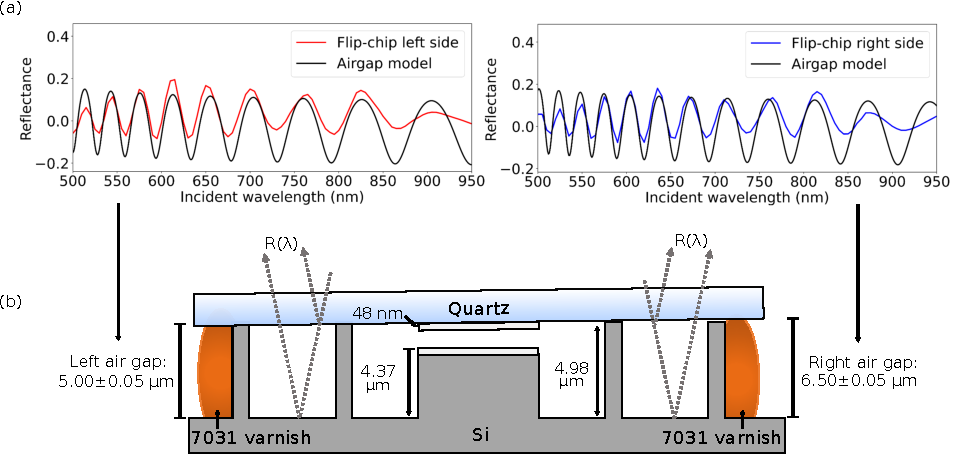
\includegraphics[width = 1\textwidth]{Flip-chip capacitor reflectance summary.pdf}
    \caption{}
    \label{FCCap Ref Summ}
\end{figure}
Figure \ref{FCCap Ref Summ} illustrates that I did not achieve parallel mounting. The left air gap agrees precisely with the etched post height of \SI{4.950(5)}{\micro\meter}; however, the right air gap sits \SI{1.50(5)}{\micro\meter} taller. The designed center gap is \SI{0.563(5)}{\micro\meter}, from AFM measurements of the posts and central mesa. Therefore, I estimate my flip-chip capacitor spacing to be \SI{1.313(55)}{\micro\meter} (\SI{0.563(5)}{\micro\meter} + \SI{1.50(5)}{\micro\meter}/2). Though I did not achieve parallel mounting, this emphasizes the strength of determining the air gap with optical methods. Before mounting the chip, wire bonding, and taking electrical measurements, the air gap of a flip-chip can be estimated, and parallel mounting can be verified. If the estimated air gap is not suitable, or the top and bottom chips are not parallel, the flip-chip can be deconstructed, cleaned, and re-mounted (7031 varnish readily dissolves in a solution of 99\% ethanol). Then, once a suitable estimated air gap is achieved, a more precise measurement can be made using capacitance.


\section{Flip-chip air gap measurement with capacitance}
The total impedance of my flip-chip capacitor is the sum of the capacitor impedance and series resistance
\begin{equation}
    Z = R_s + Z_C = R_s + \frac{1}{i\omega C}.
\end{equation}
Assume an AC signal $V = V_0 \mathrm{exp}(i\omega t)$ is applied to the flip-chip. Then, the current is 

\begin{equation} \label{current full}
    I = \frac{V}{Z} = \frac{V}{R_s + 1/i\omega C.} = V \frac{i\omega C}{1 + i\omega C R}\approx V i\omega C (1 - i\omega C R) = V(R C^2 \omega ^2 + i\omega C),
\end{equation}
where $C = \epsilon_0 A / d$ is the capacitance of the flip-chip, and I assume that the resistance is small, so $\omega C R \ll 1$. The measured current is then the real part of Eq. \ref{current full}, 

\begin{equation}
    I = V_0\omega^2 R C \mathrm{cos}(\omega t) + V_0 C \omega \mathrm{sin}(\omega t).
\end{equation}
Therefore, by applying an AC signal to the flip-chip capacitor and measuring the sine component of the resultant current, the distance between the flip-chip capacitor plates can be determined using $d = 2\pi f \epsilon_0 A V_0 / I$.

Figure \ref{FC cap measurement} (a) shows the experimental setup that I use to measure the capacitance of my flip-chip. I use a Stanford SR58 lock-in amplifier to apply a signal of $V_0 = $ \SI{100}{\milli\volt} at $f = $ \SI{200}{\hertz} and measure the sine component of the resultant current. Figure \ref{flipping chips} shows a schematic and photograph of the completed flip-chip capacitor.

\begin{figure}
    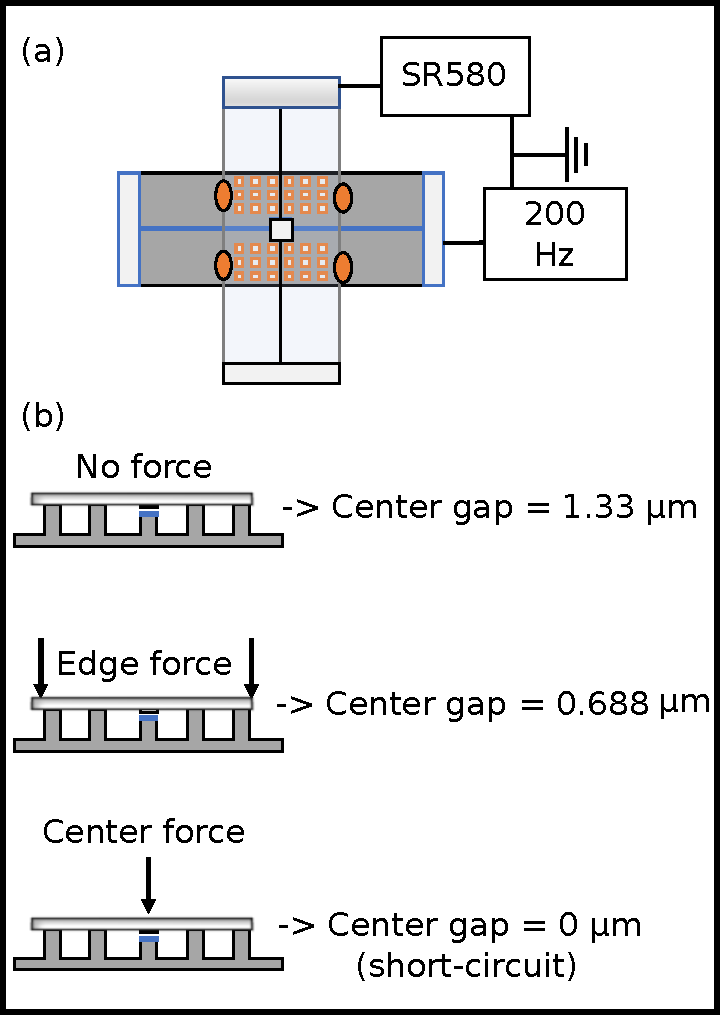
\includegraphics[width = 0.5\textwidth]{FC capacitance measurement.pdf}
    \caption{(a) schematic of the capacitance measurement. (b) Dependence of central air gap modulation with respect to location of applied mounting pressure. The edge force was applied onto the quartz chip, above the etched spacers closest to the edge of the Si chip. The central force was applied directly above the capacitor pads.}
    \label{FC cap measurement}
\end{figure}

\begin{figure}
    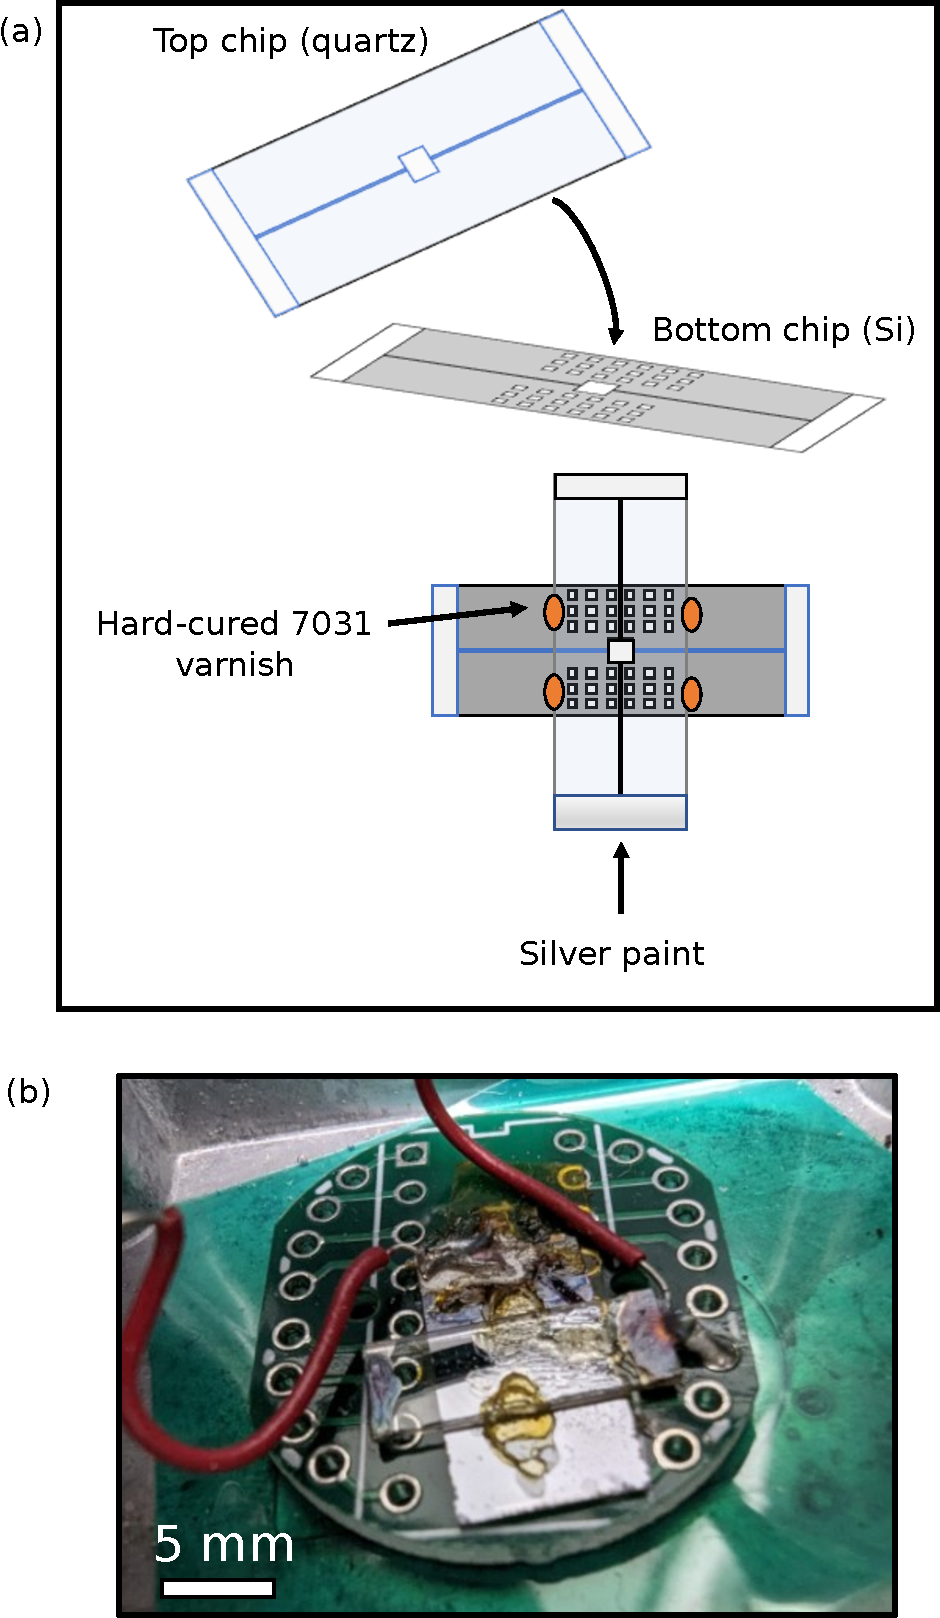
\includegraphics[width=0.5\textwidth]{flipping chips.pdf}
    \caption{(a) Schematic of the completed flip-chip capacitor. (b) Optical image of the completed flip-chip capacitor. Wires are seen soldered to the silver paint, making electrical contact to the top and bottom chips.}
    \label{flipping chips}
\end{figure}

Figure \ref{FC cap measurement} shows the results of the capacitance central air gap measurement. To determine the effect of mounting pressure, I measured the capacitance in three scenarios: applying no force, applying force on either edge of the flip-chip, and applying force in the center of the flip-chip (directly on the capacitor plates). With no mounting pressure, I determined the central air gap to be \SI{1.33(1)}{\micro\meter}, which is in very good agreement with the estimated central air gap from reflectance spectroscopy of \SI{1.36(6)}{\micro\meter} determined in Sec. \ref{FC SIspacer}. When applying edge force to simulate mechanical mounting pressure, the air gap closed to  \SI{0.688(10)}{\micro\meter}, which is close to the designed air gap defined by the etched posts (measured with AFM to be \SI{0.563(10)}{\micro\meter}). Applying a strong enough central force short-circuits the capacitor plates. 

Figure \ref{quartz bending} shows the geometry of the bent quartz chip when applying a central force to the flip-chip capacitor, short-circuiting the top and bottom chips. The bend is greatly exaggerated. Assuming that the quartz chip bends directly at the Si posts, it bends by \SI{0.563(10)}{\micro\meter} over \SI{1}{\milli\meter}, corresponding to a bending radius of \SI{0.22}{\meter} (assuming the bend forms an arc). Therefore, the strain in the quartz is \SI{0.85}{\nano\meter} / \SI{1}{\milli\meter} = $8.5 \times 10^{-5} \% $.



\begin{figure}
    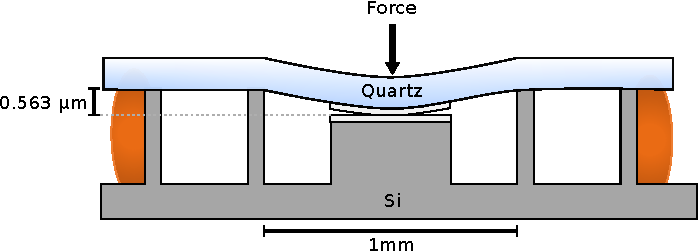
\includegraphics[width = 1\textwidth]{quartz bending.pdf}
    \caption{Geometry of the bent quartz chip with a centrally-applied force that short-circuits the top and bottom capacitor pads.}
    \label{quartz bending}
\end{figure}


\section{Conclusions}
In this section, I built a flip-chip capacitor by sandwiching patterned quartz and etched Si chips together with hard-cured varnish. I used two independent methods to characterize the gap between the two chips — interference spectroscopy ("the optical method") and capacitance. Combining both methods allows for a complete characterization of the flip-chip air gap at multiple locations, and a precise measurement between the gate chip and quantum material to be gated. The optical air gap measurement is useful for quick determination of the air gap before spending time wire bonding the chip and mounting it in a cryostat. Prior reports of flip-chip devices did not use optical methods to measure their flip-chip spacing \cite{beukman_noninvasive_2015, chu_creation_2018,satzinger_quantum_2018,bennaceur_mechanical_2015}. Using this optical method, I found that I was not able to achieve parallel mounting without external mounting pressure, likely due to the arm of my homebuilt assembly station not being perfectly level, leading to uneven mounting pressure. This is in agreement with the Si-quartz sandwiches that I created without patterned spacers (Sec. \ref{smallest achievable air gap}), in which I noticed that one side was always $\approx$ \SI{1}{\micro\meter} higher than the other, as measured using interference spectroscopy. Conversely, the capacitance measurement requires electrical contact to the chip, but can measure the air gap more precisely. The central spacing that I measured with capacitance (Fig. \ref{FC cap measurement}) in the cases of no mounting pressure and edge mounting pressure are in good agreement with the flip-chip geometry determined by AFM and optical measurement (Fig. \ref{FCCap Ref Summ}). When I applied mounting pressure to the central capacitor pads, I was able to bend the quartz chip by \SI{0.563(10)}{\micro\meter} and short-circuit the capacitor pads. This suggests the possibility of measuring the air gap of a flip-chip inside a cryostat and tuning the air gap in-situ. Future flip-chip devices could be designed with a capacitive pad in multiple locations on top and bottom chips. Then, A motorized stage inside the cryostat, such as in \cite{inbar_quantum_2023}, could be used to apply mounting pressure to the flip-chip while measuring the capacitor array to minimize the air gap and maximize the strength of coupling between the SAW gate and quantum material. 


\chapter{Conclusion}


\pagebreak

\bibliography{thesis}
\bibliographystyle{unsrt}

\pagebreak

\appendix

\chapter{Fabrication recipes}

\section{Comparison between EBL and photolithography process on LiNbO3}
\begin{itemize}
    \item \textbf{EBL process for encapsulated graphene FET on LiNbO3 with edge contacts:}
    \begin{itemize}
    \item Transfer encapsulated GR onto substrate
    \item Spin EBL resist
    \item Deposit charge dissipation layer (thin Al)
    \item Exposure (edge contact etch)
    \item Etch Al
    \item Develop resist
    \item RIE etch for edge contacts
    \item Spin EBL resist
    \item Deposit Al
    \item Exposure (contact metal)
    \item Etch Al
    \item Deposit S/D contacts
    \item Spin EBL resist
    \item Deposit Al
    \item Exposure (gate contact)
    \item Etch Al
    \item Deposit gate contact
    \end{itemize}
    \item \textbf{Photolithography process for graphene FET on LiNbO3:}
    \begin{itemize}
    \item Spin photoresist
    \item Print S/D contacts
    \item Deposit S/D contacts
    \item Transfer encapsulated GR onto substrate
    \item Spin photoresist
    \item Print gate contact
    \end{itemize}
    \end{itemize}
    

\section{Si RIE recipe}\label{Si RIE recipe}

\begin{itemize}
    \item SF\textsubscript{6}: 14.0 sccm
    \item CHF\textsubscript{3}: 35.0 sccm
    \item 100 W RF power
    \item Chamber pressure = 10 torr
    \item Si Etch rate: \SI{40}{\nano\meter/\minute}
    \item Cr etch rate: \SI{0.8}{\nano\meter/\minute}

\end{itemize}



\chapter{Additional flip-chip tests} \label{additional flip-chip tests}
I initially tried to use photoresist as spacers for flip-chip construction, following the work of \cite{bennaceur_mechanical_2015}. However, I found that the minimum spacing I could achieve was greater than a single layer of spun S1813 photoresist ($\approx$ \SI{1500}{\nano\meter}), so I transitioned to using etched Si spacers. Also, the photoresist tended to flow between the flip-chips due to capillary action, so I found that GE 7031 varnish worked much better as glue. Figure \ref{PRFC} shows my attempts at photoresist-spaced and photoresist-glued flip-chips.


\begin{figure}
    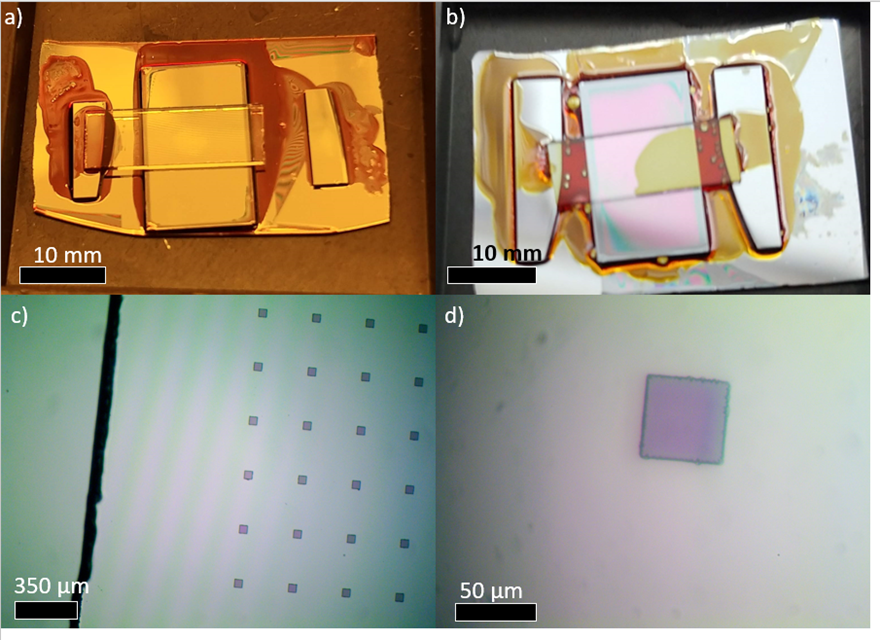
\includegraphics[width = 1\textwidth]{photoresist flip-chips.png}
    \caption{(a) A flip-chip with sandwiched quartz and Si surfaces separated by a grid of \SI{50}{\micro\meter}-wide squares spaced by \SI{350}{\micro\meter}. (b) A flip-chip where the quartz and silicon are separated by $\approx$ \SI{1}{\micro\meter} micron of spin-coated PMMA. (c) The grid of photoresist squares under quartz during alignment. (d) A single \SI{50}{\micro\meter}-wide square.
    }
    \label{PRFC}
\end{figure}

\chapter{Transferred contacts for high-quality contact to 2D semiconductors}

\chapter{Gate-tunable photoluminescence in hBN-encapsulated MoS2}

\begin{figure}
    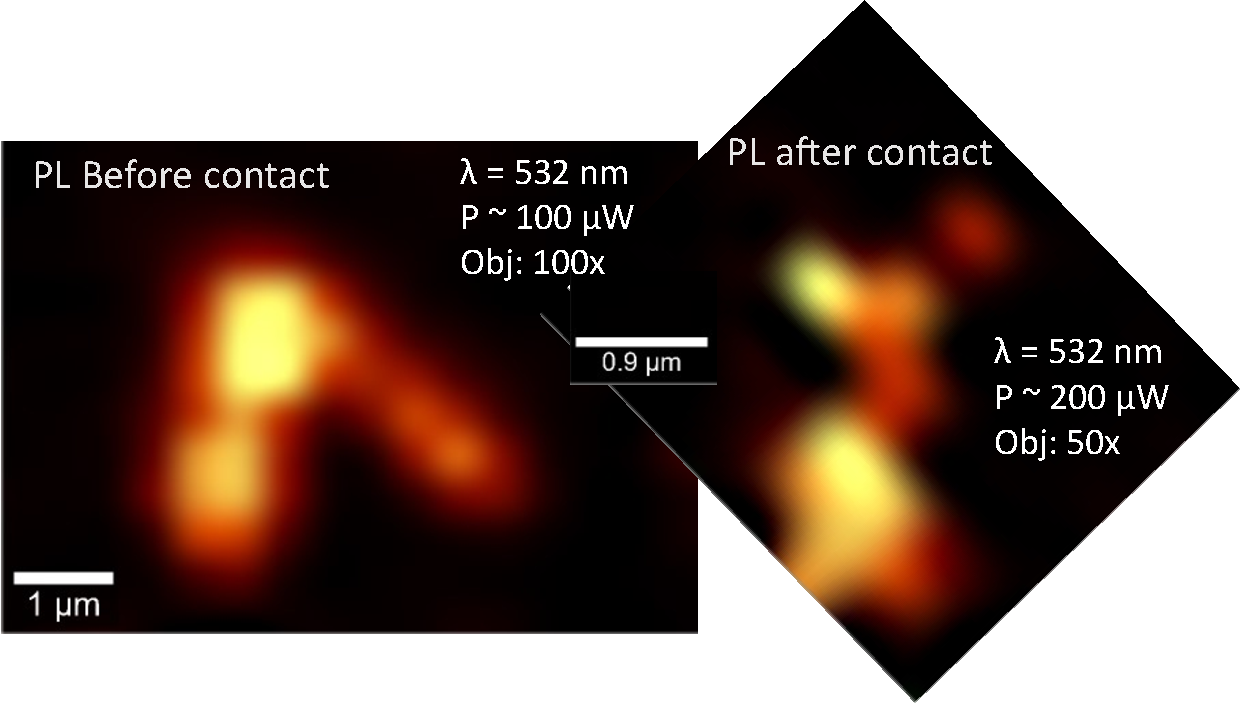
\includegraphics[width=1\textwidth]{PL before-after contact.pdf}
    \caption{}
\end{figure}

\begin{figure}
    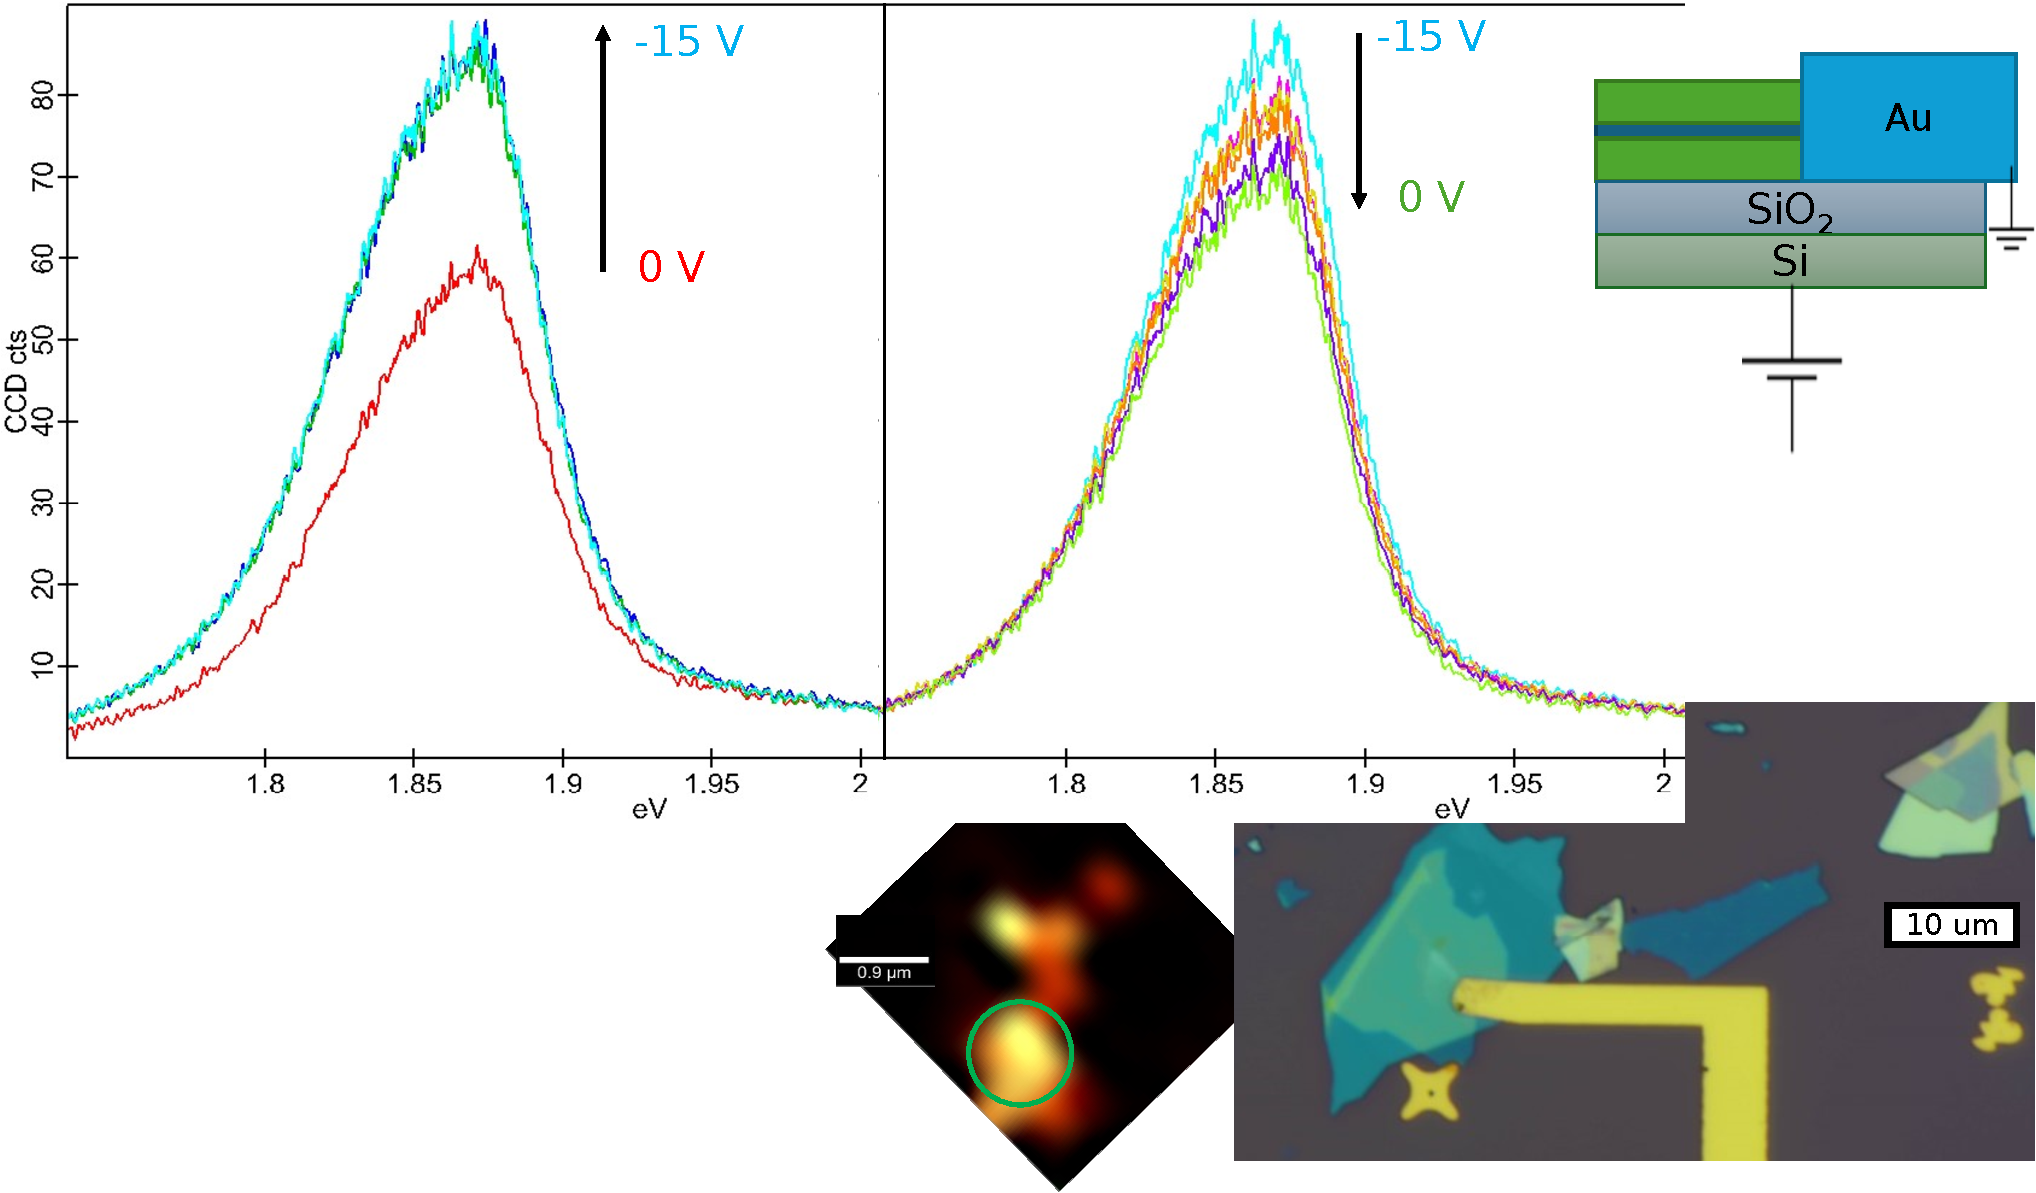
\includegraphics[width=1\textwidth]{First Vg PL sweeps.pdf}
    \caption{}
\end{figure}

\begin{figure}
    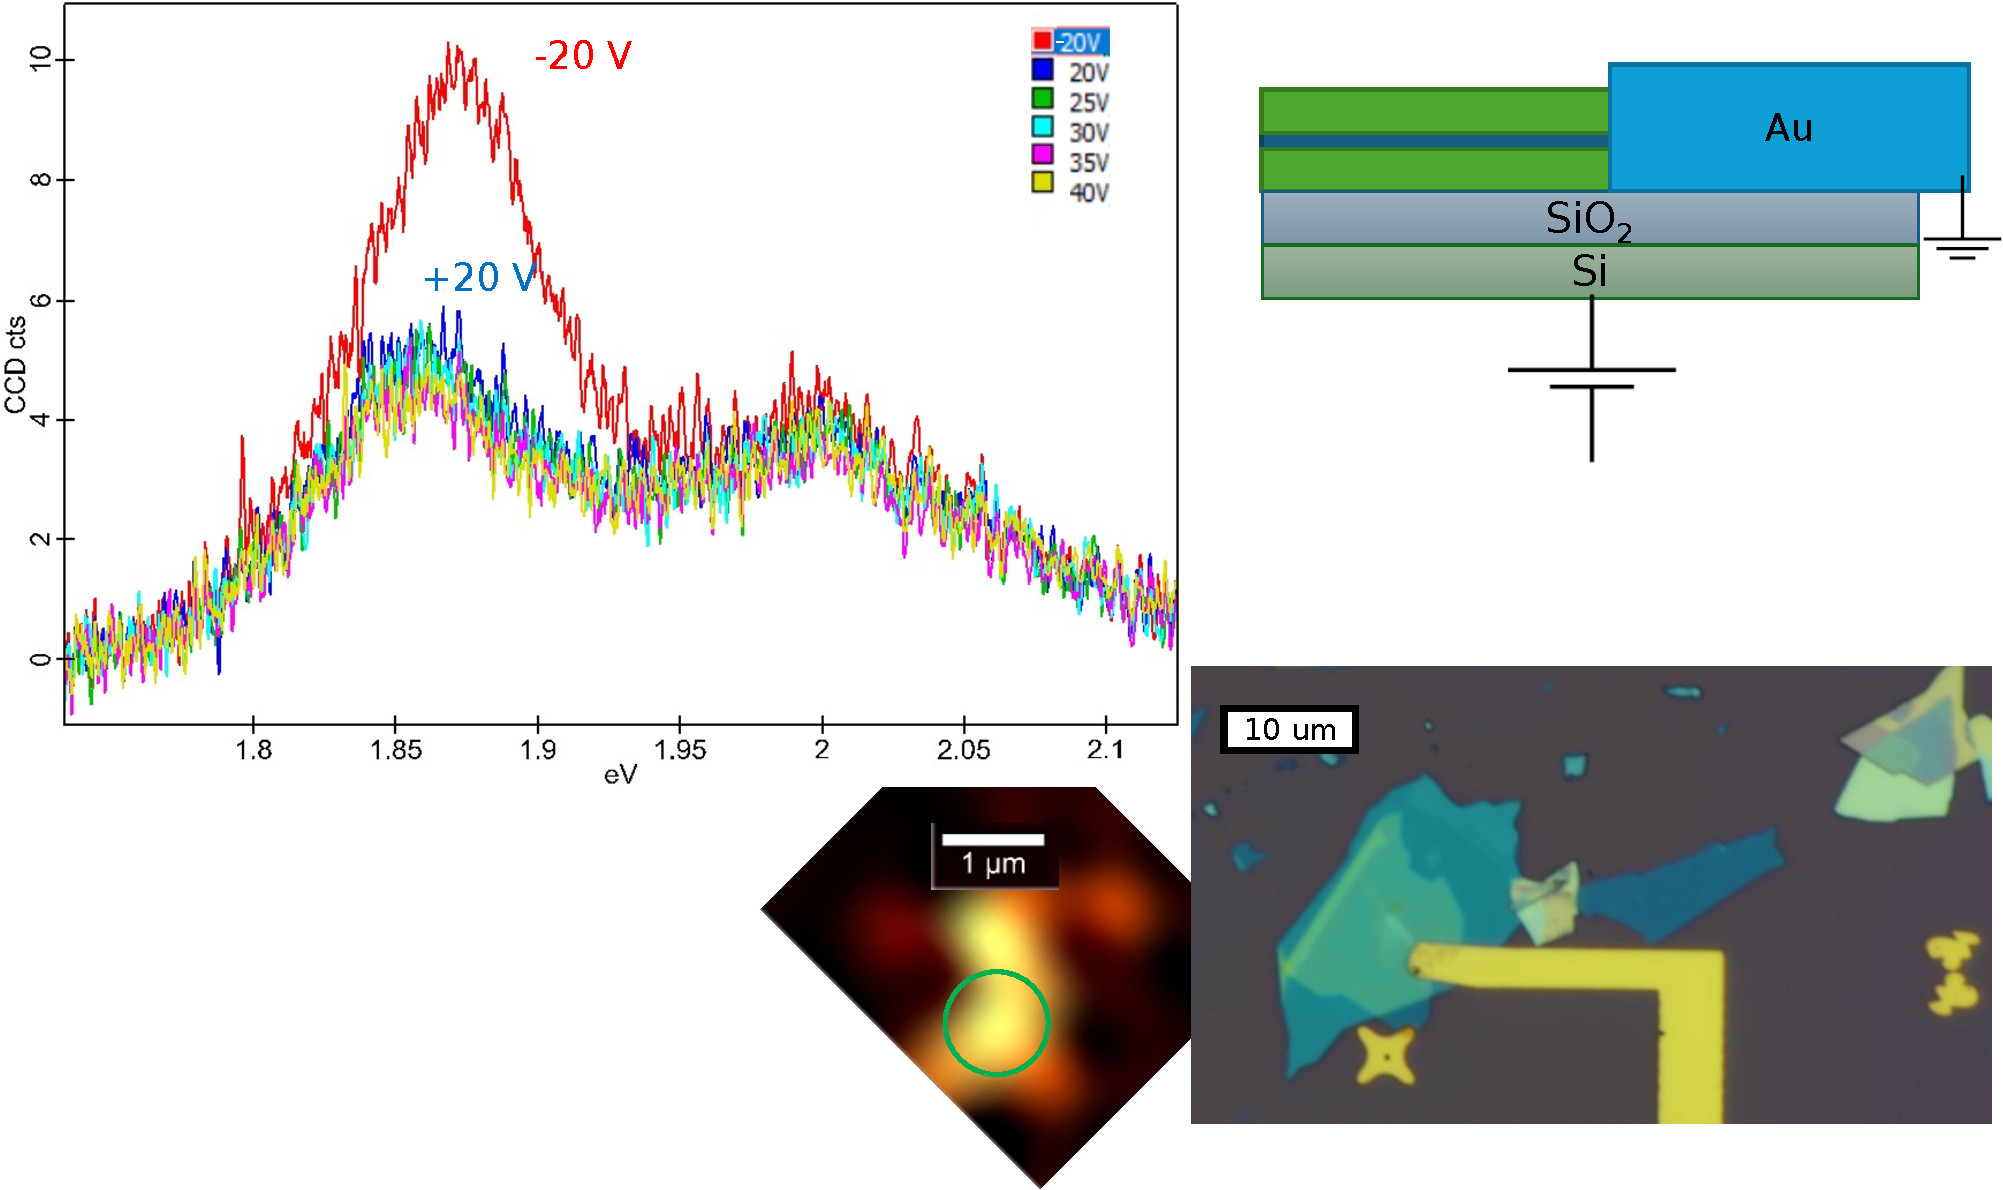
\includegraphics[width=1\textwidth]{Second Vg sweep.pdf}
    \caption{}
\end{figure}

\begin{figure}
    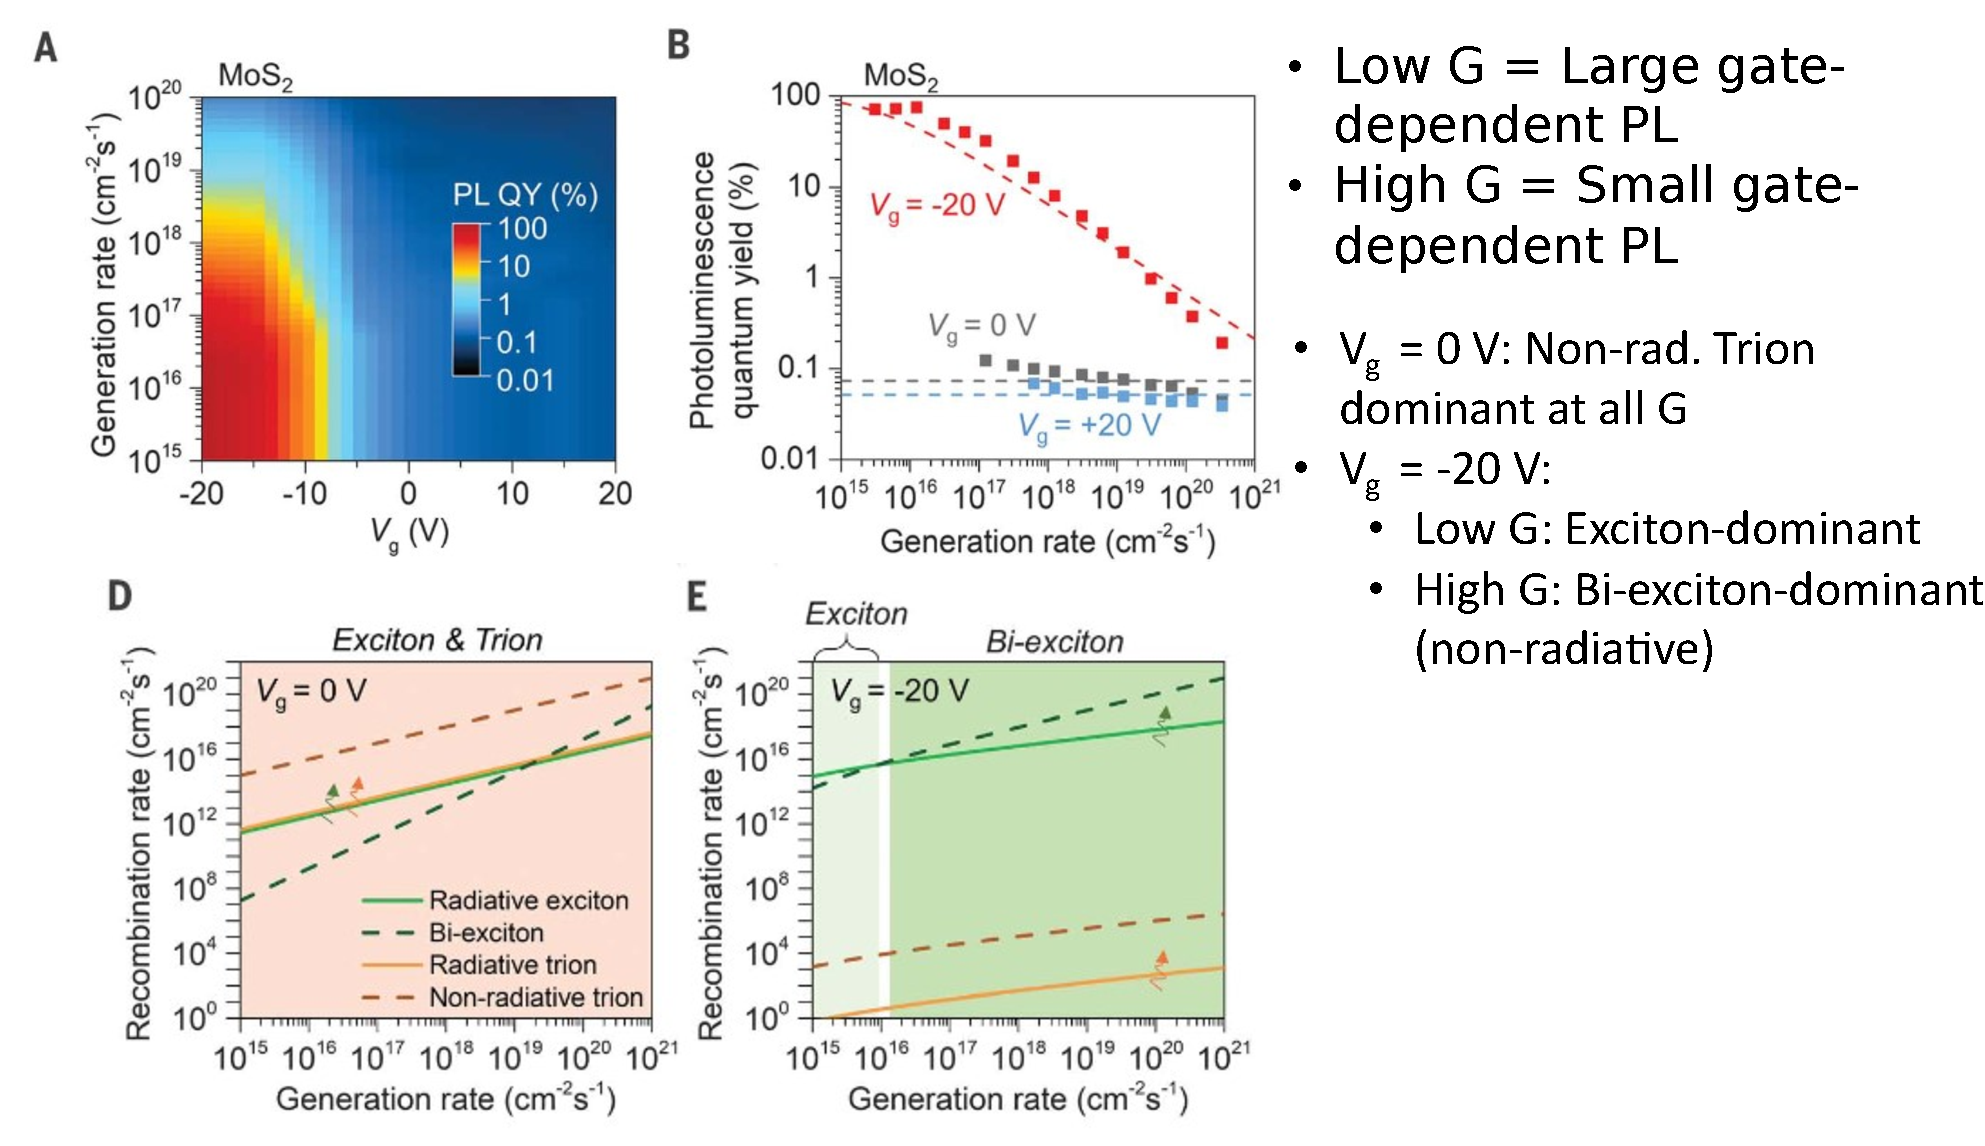
\includegraphics[width=1\textwidth]{exciton dynamics summary.pdf}
    \caption{}
\end{figure}


\end{document}